\begin{marginfigure}
  \begin{center}
    \begin{tikzpicture}
      \begin{axis}[domain=-2*3.1415:2*3.1415,
        width=7cm,height=5cm,ymin=-2.5,xmin=0,ymax=2.5,xmax=6,
        ytick={-1,1},
        yticklabels={,,},
        xticklabels={,,},
        ylabel={$x(t),{\color{blue}x[n]}$},
        xlabel=$t$, axis lines = center]
        \addplot+[ycomb,samples=15] {-0.5+sin(deg(x))+0.5*sin(2*deg(0.5*x)-0.0)+0.7*sin(3*deg(x)-0.6)+0.3*sin(4*deg(x)+1.6)};
        \addplot[samples=200]{-0.5+sin(deg(x))+0.5*sin(2*deg(0.5*x)-0.0)+0.7*sin(3*deg(x)-0.6)+0.3*sin(4*deg(x)+1.6)};
        \node at (axis cs:0.9+0.45,1.1) [above, font={\footnotesize}]{$T_s$};
        \addplot [dimen,black]plot coordinates {(0.9,1.1) (2.0*0.9,1.1)};
      \end{axis}
    \end{tikzpicture}
  \end{center}
  \caption{A continuous-time signal $x(t)$, and a discrete-time signal
    $x[n]$. Sample-spacing $T_s$ is related to sample-rate as follows:
    $T_s = 1/f_s$.}

\end{marginfigure}

This chapter introduces discrete-time signals. These are the type of
signals that are used in digital signal processing. We'll cover the
following topics:
\begin{itemize}
  \item Discretization
  \item Aliasing
  \item Oversampling and undersampling
  \item Reconstruction
  \item Shannon-Nyquist sampling theorem
\end{itemize}
In order to understand aliasing, it is important to know the
properties of complex exponential signals, as they are the natural
building blocks of signals when representing signals with the Fourier
transform. Once you understand what happens to a complex sinusoid, it
is easy to generalize what happens to all spectral components of a
signal when discretized.

\section{Sampling}
\begin{marginfigure}
  \tikzstyle{int}=[draw, minimum size=2em]
  \tikzstyle{init} = [pin edge={to-,thin,black}]
  \begin{center}
    %  \resizebox{\columnwidth}{!}{%
    \begin{tikzpicture}[every text node part/.style={align=center},node distance=3cm,auto,>=latex']
      \node [int] (a) {C-to-D \\ $T_s$};
      \node (b) [left of=a,node distance=2cm, coordinate] {a};
      %    \node (c) [below=a,node distance=3cm] {a};

      %\node [int, pin={[init]above:$p_0$}] (c) [right of=a] {$\frac{1}{s}$};
      \node [coordinate] (end) [right of=a, node distance=3cm]{};
      \path[->] (b) edge node {$x(t)$} (a);
      %\path[->] (a) edge node {$v$} (c);
      \draw[->] (a) edge node {$x[n]=x(nT_s)$} (end) ;
    \end{tikzpicture}
    % }
  \end{center}
  \caption{An ideal continuous-time to Discrete-time (C-to-D) converter.}
\end{marginfigure}

A continuous-time signal can be converted into a discrete-time signal
by sampling it. This can be seen as a operation that selects evenly
space values of a continuous-time signal:
\begin{equation}
  \boxed{
    x[n] = x(n T_s)
  }\,\,.
\end{equation}
In this process, a continuous function $x(t) \in \mathbb{C}$ is
converted into an ordered sequence of numbers $x[n] \in \mathbb{C}$,
where $n\in\mathbb{Z}$ indicates the order of the numbers.

The reason why we consider complex-valued signals in addition to
real-valued signals is that there are many applications where the
signals are naturally complex-valued.  Radio signal processing is one
example. Real valued signals are a subset of complex valued signals,
and thus, the theory also applies to such signals as well.

The \index{sample-spacing}{sample-spacing} $T_s$ determines how
densely samples of the continuous-time signal are
taken. Sample-spacing is related with the
\index{sample-rate}{sample-rate} or
\index{sampling-rate}{sampling-rate} $f_s$ as follows:
\begin{equation}
  \boxed{
    f_s = \frac{1}{T_s}
  }\,\,.
\end{equation}
Sample-rate typically is given in units of samples per second or
\emph{\index{hertz}{hertz}} when the independent variable is time. In
other cases, many other possibilities also exist. For example, the
resolution of a digital image is often given in units of dots per inch
(DPI).

\if 0 You can think of sampling as a convolution operation between a
  time-shifted unit impulse $\delta(t-nT_s)$ and the continuous-time
  signal $x(t)$:
  \begin{align}
    x[n] & = \int_{-\infty}^{\infty} x(\tau) \delta(n T_s - \tau)  d\tau \\
         & = x(n T_s)\,\,.
  \end{align}
\fi

\subsection{Sampling a complex sinusoidal signal}

The key to understanding the concept of aliasing when discretizing signals is to study how a complex sinusoidal signal behaves when it is discretized:
\begin{equation}
  x(t)=A e^{i\phi} e^{i\omega_0 t}\,\,.
\end{equation}
Because we can use the Fourier transform to represent continuous-time
signals as sums of complex sinusoidal signals, knowledge of what
happens to a single complex sinusoidal signal can be generalized to
arbitrary signals, by studying what happens to each spectral component
of a signal.

\begin{marginfigure}
  \begin{center}
    \begin{tikzpicture}
      \begin{axis}[width=7cm,height=6cm,ymin=0,xmin=-3,ymax=1.5,xmax=3,  yticklabels={,,},
          xtick={1.0},
          ylabel={$\hat{x}(\omega)=Ae^{i\phi}\delta(\omega-\omega_0)$},
          xticklabels={$\omega_0$},
          xlabel=$\omega$, axis lines = center]
%+[dirac]
        \addplot + [dirac] plot coordinates {(1,1)};
%        \node at (axis cs:1,1.1) [above, font={\footnotesize}]{$Ae^{i\phi}\delta(\omega-\omega_0)$};
      \end{axis}
    \end{tikzpicture}
  \end{center}
  \caption{The Fourier transform representation of a complex sinusoidal signal.}
\end{marginfigure}

So what happens to a complex sinusoidal signal when we sample it?
\begin{align}
  x[n] & =x(nT_s)                                \\
       & =A e^{i\phi} e^{i\omega_0 n T_s }       \\
       & =A e^{i\phi} e^{i\hat{\omega}_0 n}\,\,.
\end{align}
What happens is that we get a discrete-time complex sinusoidal signal. This signal has a special type of frequency:
\begin{equation}
  \boxed{
    \hat{\omega}_0 = \omega_0 T_s
  }\,\,.
\end{equation}

The angular frequency $\hat{\omega}_0$ is called a
\emph{\index{discrete-time angular frequency}{discrete-time angular
  frequency}}.  It indicates how many \emph{\index{radians per
  sample}{radians per sample}} the phase of the complex sinusoidal
signal advances. With a discrete-time signal, time is only implied
from the sample spacing that was used to discretize the signal, which
is why no time unit is attached to $\hat{\omega}_0$. There's a hat on
$\hat{\omega}_0$ to signify that this is not the same kind of
frequency as the continuous-time angular frequency $\omega$, which has
units of radians per second.

Figure \ref{fig:rotating_dt_phasor} shows an example of how the values of the discrete-time complex 
sinusoidal signal behave with increasing sample index, obtaining values on a circle of 
radius $A$ in the complex plane. The amount of angle per sample that the signal advances for
each sample on the circle is given by the discrete-time angular frequency $\hat{\omega}_0$.

\begin{marginfigure}
  \begin{center}
    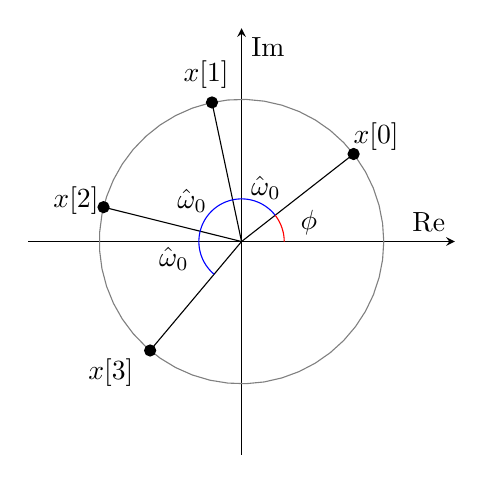
\begin{tikzpicture}
      \pgfmathsetmacro{\PHI}{38}
      \pgfmathsetmacro{\OM}{64}
      \begin{axis}[axis equal, disabledatascaling,
          ymin=-1.5,xmin=-1.5,ymax=1.5,xmax=1.5, ticks=none,
          xlabel=$\mathrm{Re}$, ylabel=$\mathrm{Im}$, axis lines = center,
          width=7cm, height=7cm]
        % unit circle
        \addplot [gray,domain=0:2*pi,samples=50]({cos(deg(x))},{sin(deg(x))});
        % first sample
        \addplot [black, mark = *] coordinates {( {cos(\PHI)}, {sin(\PHI)} )} {};
        \addplot [black] coordinates { (0,0) ( {cos(\PHI)}, {sin(\PHI)} ) };

        % second sample
        \addplot [black, mark = *] coordinates {( {cos(\OM+\PHI)}, {sin(\OM+\PHI)} )} {};
        \addplot [black] coordinates { (0,0) ( {cos(\OM+\PHI)}, {sin(\OM+\PHI)} ) };

        % third sample
        \addplot [black, mark = *] coordinates {( {cos(2*\OM+\PHI)}, {sin(2*\OM+\PHI)} )} {};
        \addplot [black] coordinates { (0,0) ( {cos(2*\OM+\PHI)}, {sin(2*\OM+\PHI)} ) };

        % third sample
        \addplot [black, mark = *] coordinates {( {cos(3*\OM+\PHI)}, {sin(3*\OM+\PHI)} )} {};
        \addplot [black] coordinates { (0,0) ( {cos(3*\OM+\PHI)}, {sin(3*\OM+\PHI)} ) };

        \node at (axis cs:{1.2*cos(\PHI)},{1.2*sin(\PHI)}) {$x[0]$};
        \node at (axis cs:{1.2*cos(\OM+\PHI)},{1.2*sin(1*\OM+\PHI)}) {$x[1]$};
        \node at (axis cs:{1.2*cos(2*\OM+\PHI)},{1.2*sin(2*\OM+\PHI)}) {$x[2]$};
        \node at (axis cs:{1.2*cos(3*\OM+\PHI8)},{1.2*sin(3*\OM+\PHI)}) {$x[3]$};


        \addplot [red,domain=0:(pi*\PHI/180),samples=50]({0.3*cos(deg(x))},{0.3*sin(deg(x))});
        \node at (axis cs:{0.5*cos(\PHI/2.0)},{0.4*sin(\PHI/2.0)}) {$\phi$};

        \addplot [blue,domain=(pi*\PHI/180):(pi*(\PHI+\OM)/180),samples=50]({0.3*cos(deg(x))},{0.3*sin(deg(x))});
        \node at (axis cs:{0.5*cos((\PHI+\PHI+\OM)/2)},{0.4*sin((\PHI+\PHI+\OM)/2)}) {$\hat{\omega}_0$};

        \addplot [blue,domain=(pi*(\PHI+\OM)/180):(pi*(\PHI+2*\OM)/180),samples=50]({0.3*cos(deg(x))},{0.3*sin(deg(x))});
        \node at (axis cs:{0.5*cos((\PHI+\OM + \PHI+2*\OM)/2)},{0.4*sin((\PHI+\OM + \PHI+2*\OM)/2)}) {$\hat{\omega}_0$};

        \addplot [blue,domain=(pi*(\PHI+2*\OM)/180):(pi*(\PHI+3*\OM)/180),samples=50]({0.3*cos(deg(x))},{0.3*sin(deg(x))});
        \node at (axis cs:{0.5*cos((\PHI+2*\OM + \PHI+3*\OM)/2)},{0.4*sin((\PHI+2*\OM + \PHI+3*\OM)/2)}) {$\hat{\omega}_0$};

      \end{axis}
    \end{tikzpicture}
  \end{center}
  \caption{A discretized complex sinusoidal signal $x[n] = A e^{i\phi}e^{i\hat{\omega}_0n}$ 
  with phase increments of $\hat{\omega}_0$ radians per sample. The initial phase for sample $n=0$ is given by $\phi$.}
  \label{fig:rotating_dt_phasor}
\end{marginfigure}

\subsection{Frequency aliases}

What happens if $\hat{\omega}$ is larger than $2\pi$? In this case,
the phasor rotates around the circle on the complex plane more than
once for times every sample. It is easy to convince yourself that this
can lead to ambiguity. There are infinitely many values of
$\hat{\omega}$ that describe an identical complex sinusoidal
sginal. This phenomenon is called aliasing.

Aliases of a signal mean all the possible values of $\hat{\omega}$ that
result in an identical complex sinusoidal signal:
\begin{align}
  x[n] & =Ae^{i\phi} e^{i(\hat{\omega}_0 + 2\pi k) n} \\
       & =Ae^{i\phi} e^{i \hat{\omega}_0  n}
\end{align}
where $k\in\mathbb{Z}$. What this means is that we can select any one
of the discrete-time angular frequencies:
\begin{equation}
  \boxed{
    \hat{\omega}_k = \hat{\omega}_0 + 2\pi k
  }\,\,.
\end{equation}
and our discrete-time complex sinusoidal signal will be
identical. These discrete-time angular frequencies $\hat{\omega}_k$
are called \emph{\index{aliases}{aliases}}.


\begin{marginfigure}[5cm]
  \begin{center}
    \begin{tikzpicture}
      \begin{axis}[
          width=7cm,
          height=6cm,
          ymin=0,
          xmin=-4,
          ymax=1.2,
          xmax=4,
          yticklabels={,,},
          xtick={-3.6,-1.6, .4, 2.4},
          xticklabels={$f_0-2 f_s $,$f_0- f_s$,$f_0$,$f_0+f_s$},
          xlabel=$f$,
          ylabel=$\hat{x}(f)$,
          axis lines = center]
        \addplot+[dirac] plot coordinates {((-3.6,1) (-1.6,1) (0.4,1) (2.4,1)};
      \end{axis}
    \end{tikzpicture}
  \end{center}
  \caption{Each one of these signals $Ae^{i\phi}e^{i2\pi (f_0 + k f_s)t}$
  would result in the same discrete-time complex sinusoidal signal
  when discretized with sample-rate $f_s$. Note that we're showing the
  spectrum with continuous-time frequency in units of hertz (cycles
  per second) instead of radians per second.}
\end{marginfigure}

Using just the discrete-time signal complex sinusoid, there is no way
of telling what is the true continuous-time angular frequency that
produced our discrete-time signal. What continuous-time frequencies do
these aliases correspond to? We can work this out by looking at the
continuous-time complex sinusoidal signal of frequency $\omega_0$:
\begin{equation}
  x(t) = A e^{i\phi} e^{i\omega_0 t}\,\,.
\end{equation}
When discretized, each of the following signals are identical:
\begin{align}
  x[n] & =A e^{i\phi} e^{i \omega_0 T_s n }                \\
       & = A e^{i\phi} e^{i(\omega_0 T_s + 2\pi k) n }     \\
       & = A e^{i\phi} e^{i(\omega_0 + 2\pi k/T_s) T_s n } \\
       & = A e^{i\phi} e^{i(\omega_0 + 2\pi k f_s) T_s n } \\
       & = A e^{i\phi} e^{i \omega_k T_s n } \,\,.
\end{align}
We've used the relationship between sample-rate $f_s=1/T_s$ and sample
spacing here. The aliases map to continuous-time angular frequency as
follows:
\begin{equation}
  \boxed{
    \omega_k = \omega_0 + 2\pi k f_s
  }\,\,
\end{equation}

Any one of these continuous-time angular frequencies $\omega_k$ would
result in an identical discrete-time complex sinusoidal signal when
discretized with sample-rate $f_s$. Dividing by
$2\pi$, we get the aliasing behavior in units of hertz (samples per
second)\footnote{remember that angular frequency (radians per second)
  and frequency (cycles per second) are related as follows $\omega = 2\pi
    f$.}:
\begin{equation}
  \boxed{
    f_k = f_0 + k f_s
  }\,\,.
\end{equation}
The phenomena of aliasing is problematic. We cannot uniquely
distinguish a discrete-time complex sinusoidal signal
$x[n]=Ae^{i\hat{\omega}n}$ which continuous-time signal it corresponds
to. Conversely, there are infinitely many continuous-time sinusoidal
signals $x(t)=Ae^{i\omega t}$ that will result in the same
discrete-time signal. In order to resolve this ambiguity, we need a
priori information about the spectral occupancy of the continuous-time
signal.

\begin{marginfigure}
  \begin{center}
    \begin{tikzpicture}
      \begin{axis}[domain=-6:6,
          width=7cm,height=6cm,ymin=-1.2,xmin=-4,ymax=1.4,xmax=4,
          ytick={-1,1},
          yticklabels={$-A$, $A$},
          xlabel=$t$, axis lines = center]
        \addplot+[ycomb,samples=15,color=blue]{cos(deg(2.0*3.1415*1.35*x+3.14/4))};
        \addplot+[ycomb,samples=15,color=red]{sin(deg(2.0*3.1415*1.35*x+3.14/4))};

        \addplot[samples=400,blue]{cos(deg(2.0*3.1415*1.35*x+3.14/4))};
        \addplot[samples=400,red]{sin(deg(2.0*3.1415*1.35*x+3.14/4))};
        %            \addplot[samples=400,color=red]{cos(deg(2.0*3.1415*0.18333333333333335*x+3.14/4))};
        %           \addplot[samples=400,color=green]{cos(deg(2.0*3.1415*0.9833333333333334*x-3.14/4))};


        \node  at (axis cs:0.9+0.45,1.1) [above, font={\footnotesize}]{$T_s$};
        \addplot [dimen,black]plot coordinates {(0.9,1.1) (2.0*0.9,1.1)};
      \end{axis}

    \end{tikzpicture}
    \begin{tikzpicture}
      \begin{axis}[domain=-6:6,
          width=7cm,height=6cm,ymin=-1.2,xmin=-4,ymax=1.4,xmax=4,
          ytick={-1,1},
          yticklabels={$-A$, $A$},
          xlabel=$t$, axis lines = center]
        %            \addplot[samples=400,blue]{cos(deg(2.0*3.1415*1.35*x+3.14/4))};
        \addplot+[ycomb,samples=15,color=blue]{cos(deg(2.0*3.1415*0.18333333333333335*x+3.14/4))};
        \addplot+[ycomb,samples=15,color=red]{sin(deg(2.0*3.1415*0.18333333333333335*x+3.14/4))};
        \addplot[samples=400,color=blue]{cos(deg(2.0*3.1415*0.18333333333333335*x+3.14/4))};
        \addplot[samples=400,color=red]{sin(deg(2.0*3.1415*0.18333333333333335*x+3.14/4))};
        %            \addplot[samples=400,color=green]{cos(deg(2.0*3.1415*0.9833333333333334*x-3.14/4))};


        \node  at (axis cs:0.9+0.45,1.1) [above, font={\footnotesize}]{$T_s$};
        \addplot [dimen,black]plot coordinates {(0.9,1.1) (2.0*0.9,1.1)};
        %\addplot[color=black] plot coordinates {(0.9,1.1) (2.0*0.9,1.1)};
      \end{axis}
    \end{tikzpicture}
  \end{center}
  \caption{Two different complex sinusoidal signals that result in the same discrete-time signal.}
\end{marginfigure}

Solving the problem of aliasing, by ensuring that there is a uniquely one-to-one mapping 
between continuous-time and discrete-time frequencies for all the spectral components 
of a signal, leads to the Shannon-Nyquist sampling theorem, which is introduced at the end of this chapter.

\subsection{Real-valued sinusoids}

With knowledge of how a complex sinusoidal signal is aliased, we can
inspect how real-valued sinusoidal signals behave when discretized. We
know using Euler's formula that real valued sinusoidal signals are a
sum of two complex exponential signals. This is only slightly more
complicated than the previous case.

\if 0
The Fourier transform of a real-valued signal $x(t)\in\mathbb{R}$ is
conjugate symmetric
\begin{equation}
  \hat{x}(\omega) = \hat{x}^*(-\omega)\,\,.
\end{equation}
\fi 
Recall that:
\begin{equation}
  A \cos(\omega t + \phi) = \frac{A}{2}(e^{i\phi}e^{i\omega t} + e^{-i\phi}e^{-i\omega t})\,\,.
\end{equation}
In order to understand how aliasing affects real-valued sinusoids, we
need to investigate how pairs of positive and negative frequency
spectral components are affected.
\begin{marginfigure}
  \begin{center}
    \begin{tikzpicture}
      \begin{axis}[width=7cm,height=6cm,ymin=0,xmin=-2,ymax=1.5,xmax=2,  yticklabels={,,},
          xtick={-1, 1.0},
          xticklabels={$-\omega_0$,$\omega_0$},
          ylabel=$\hat{x}(\omega)$,
          xlabel=$\omega$,
          axis lines = center]

        \addplot+[ycomb] plot coordinates {(1,1)};
        \addplot+[ycomb] plot coordinates {(-1,1)};

        \node at (axis cs:1,1.1) [above, font={\footnotesize}]{$\frac{A}{2}e^{i\phi}$};
        \node at (axis cs:-1,1.1) [above, font={\footnotesize}]{$\frac{A}{2}e^{-i\phi}$};
      \end{axis}
    \end{tikzpicture}
  \end{center}
  \caption{A real-valued signal consists of a positive and negative frequency spectral component, 
  which are conjugate symmetric.}
\end{marginfigure}
A conjugate symmetric pairing of positive and negative frequencies
means that there is no distinction between a positive and a negative
frequency signal\footnote{For complex sinusoidal signals $e^{-i \omega
  t}$ and $e^{i \omega t}$ are two unique signals.}.  For example,
let's say we have a signal with angular frequency $\omega = -0.1$:
\begin{equation}
  A \cos(-0.1 t + \phi) = \frac{A}{2}(e^{i\phi}e^{-i0.1  t} + e^{-i\phi}e^{i0.1 t})\,\,.
\end{equation}
This is the same thing as a cosine signal with frequency $0.1$, but a
sign flipped phase:
\begin{align}
  \frac{A}{2}(e^{-i\phi}e^{i 0.1 t} + e^{i\phi}e^{-i 0.1 t}) & = A \cos(0.1 t - \phi)       \\
                                                             & = A \cos(-0.1 t + \phi)\,\,.
\end{align}
This means that you can always represent a real-valued sinusoidal
signal using only positive valued frequencies. This results in more
complicated aliasing behaviour!

In the case of real-valued sinusoids, the frequency alias
corresponding to a negative frequency is called a \emph{\index{folded
  alias}{folded alias}}.

\subsection{Example: Sinusoidal signal with $f_0=1$ Hz and $f_s=10$ Hz}
\begin{marginfigure}
  \begin{center}
    \includegraphics[width=\textwidth]{code/014_sampling/aliased_signals.png}
  \end{center}
  \caption{Example of signal aliasing for $f_0\in \{-19,-9,1,11,21\}$
    Hz and $f_s=10$ Hz. All signals alias identically. Python code:
    \texttt{014\_sampling/aliasing\_example.py}.}
\end{marginfigure}

Consider the following sinusoidal signal with a frequency of $f_0 =1$ Hz and phase $\phi$:
\begin{align}
  x(t) & =A\cos(2\pi f_0 t + \phi)  \\
  x(t) & =A\cos(2\pi t + \phi)\,\,.
\end{align}
When discretized with a sample-rate $f_s=10$ Hz or $T_s=1/f_s = 0.1$ s this becomes:
\begin{align}
  x[n] & =x(nT_s)                     \\
       & =A\cos(2\pi n T_s + \phi),   \\
       & =A\cos(0.2\pi n + \phi)\,\,.
\end{align}
The discrete-time angular frequency is $\hat{\omega}_0 = 0.2\pi$. 
For any $k\in\mathbb{Z}$ this signal is identical to:
\begin{align}
  x[n] & =A\cos([0.2\pi + 2\pi k] n + \phi)\,\,.
\end{align}
In discrete-time angular frequencies (radians per sample), the aliases are:
\begin{align}
  \hat{\omega}_k & = (0.2\pi+2\pi k)                                   \\
                 & =\ldots,-3.8\pi,-1.8\pi,0.2\pi,2.2\pi,4.2\pi,\ldots
\end{align}
In continuous-time frequency (Hz), the aliases would be:
\begin{align}
  f_k & =f_0 + f_s k                     \\
      & =\ldots,-19,-9,1,11,21,31,\ldots
\end{align}
In other words, a discretized cosine signal produced from any of the frequencies $f_k$ 
would be identical to a 1 Hz signal, when using 10 Hz sample rate. The negative solutions 
are called folded aliases, which can be interpreted as cosine signals with positive 
frequencies $9,19,\cdots$ but with a sign flipped phase.

\begin{figure}
  \begin{center}
    \begin{tikzpicture}
      \begin{axis}[
          domain=-6:6,
          width=12cm,
          height=6cm,
          ymin=-1.2,
          xmin=-4,
          ymax=1.4,
          xmax=4,
          ytick={-1,1},
          yticklabels={$-A$, $A$},
          xlabel=$t$,
          axis lines = center]
        \addplot[samples=400,blue]{cos(deg(2.0*3.1415*1.35*x+3.14/4))};
        \addplot+[ycomb,samples=15,color=red]{cos(deg(2.0*3.1415*1.35*x+3.14/4))};
        \addplot[samples=400,color=red]{cos(deg(2.0*3.1415*0.18333333333333335*x+3.14/4))};
        \addplot[samples=400,color=green]{cos(deg(2.0*3.1415*0.9833333333333334*x-3.14/4))};

        \node at (axis cs:0.9+0.45,1.1) [above, font={\footnotesize}]{$T_s$};
        \addplot[dimen,color=black] plot coordinates {(0.9,1.1) (2.0*0.9,1.1)};
      \end{axis}
    \end{tikzpicture}
  \end{center}
  \caption{The following figure illustrates what the continuous-time and discrete-time signals 
  look like. They are all identical in discrete-time, because the continuous-time signals 
  intersect at the sampling points. The red line shows $\omega_0 = 0.2\pi f_s$ (1 Hz), 
  the green line shows $\omega_1 = -1.8\pi f_s$ (-9 Hz), and the blue line shows $\omega_2=2.2\pi f_s$ (11 Hz).
  One can also see the phase-flip on the negative frequency folded alias, shown in green.
  The blue and red continuous-time signals are both sampled at identical phases, but the green not.}
\end{figure}

Figure \ref{fig:dt_spec_ex} shows part of the discrete-frequency
spectrum where there are three aliases of the cosine signal. There are infinitely many aliases, but only three are shown here.
It is customary to call the region of the spectrum where $|\hat{\omega}| < \pi$ or $|f| < f_s/2$, the \emph{principal spectrum}.
This region of the spectrums contains the smallest discrete-time angular frequency aliases.
\begin{figure}
  \begin{center}
    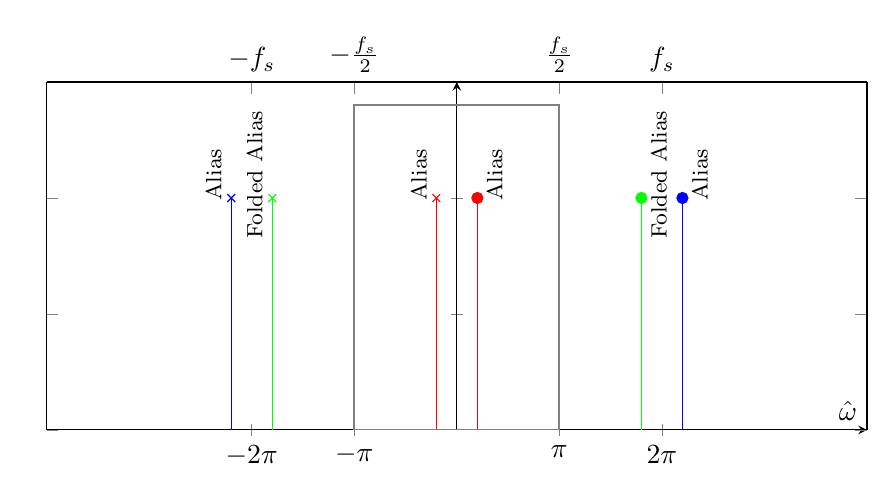
\begin{tikzpicture}
      \begin{axis}[width=12cm,height=6cm,ymin=0,xmin=-4,ymax=1.5,xmax=4,  yticklabels={,,},
          xtick={-2,-1,1,2},
          xticklabels={$-2\pi$,$-\pi$,$\pi$,$2\pi$},
          xlabel=$\hat{\omega}$, axis lines = center]

        \addplot[ycomb,color=blue,mark=*,mark color=blue] plot coordinates {(2.2,1)};
        \addplot[ycomb,color=green,mark=*,mark color=green] plot coordinates { (1.8,1)};
        \addplot[ycomb,color=red,mark=*,mark color=red] plot coordinates { (0.2,1)};

        \addplot[ycomb,color=blue,mark=x,mark color=blue] plot coordinates {(-2.2,1)};

        \addplot[ycomb,color=green,mark=x,mark color=green] plot coordinates {(-1.8,1)};

        \addplot[ycomb,color=red,mark=x,mark color=red] plot coordinates {(-0.2,1)};

        \node at (axis cs:0.2,1.1) [below, rotate=90, font={\footnotesize}]{Alias};
        \node at (axis cs:-0.2,1.1) [above, rotate=90, font={\footnotesize}]{Alias};
        \node at (axis cs:1.8,1.1) [below, rotate=90, font={\footnotesize}]{Folded Alias};
        \node at (axis cs:-1.8,1.1) [above, rotate=90, font={\footnotesize}]{Folded Alias};

        \node at (axis cs:2.2,1.1) [below, rotate=90, font={\footnotesize}]{Alias};
        \node at (axis cs:-2.2,1.1) [above, rotate=90, font={\footnotesize}]{Alias};

        \draw [gray, thick] (axis cs:-1,0.0) rectangle (axis cs:1,1.4);
      \end{axis}
      \begin{axis}[
          width=12cm,
          height=6cm,
          ymin=0,
          xmin=-4,
          ymax=1.5,
          xmax=4,
          yticklabels={,,},
          xlabel={},
          xtick={-2,-1,1,2},
          xticklabels={$-f_s$,$-\frac{f_s}{2}$,$\frac{f_s}{2}$,$f_s$},
          axis x line*=top]

      \end{axis}
    \end{tikzpicture}
  \end{center}
  \caption{Spectral aliases of the components plotted as a function of
    discrete-time angular frequency $\hat{\omega}$ (radians per
    sample). The pairing of positive and negative frequencies indicates
    that this signal is real-valued, and that the $\hat{\omega}_{-1} =
      -1.8\pi$ alias corresponds to a cosine signal with a positive
    discrete-time angular frequency of $1.8\pi$ and a flipped
    phase. Frequency in units of hertz is shown on the top axis.}
  \label{fig:dt_spec_ex}
\end{figure}

How could we be able to determine which one of the frequencies $f_k$
is the true sinusoidal frequency component represented by the
discrete-time signal? We can only do this if we know that the
continuous-time frequencies of the spectral components of the signal
lie within a certain range.

For example, if we knew that there are no spectral components with
frequencies higher than 5 Hz present in the continuous-time signal
($|f| < 5$) Hz, then we could determine that the discrete-time signal
is due to a 1 Hz continuous-time signal, because this is the only
possible mapping between a discrete-time frequency and a
continuous-time frequency.

\subsection{Principal spectrum}
The \emph{\index{principal spectrum}{principal spectrum}} (also called normalized angular frequency) 
is the range of discrete-time angular frequencies between:
\begin{equation}
  \boxed{-\pi < \hat{\omega} < \pi}\,\,.
\end{equation}
It is the region for the lowest frequency discrete-time angular
frequency representation for discrete-time spectral components that
the signal consists of.  Unaliased continuous-time frequencies between
\begin{equation}
  -f_s/2 < f < f_s/2
\end{equation}
in units of hertz are mapped to this range of discrete-time angular
frequencies.

By finding a suitable value for $k$, it is possible to find an alias
of any discrete-time angular frequency $\hat{\omega}$, which lands in
the range $-\pi< \hat{\omega}+2\pi k < \pi$. This is called the
\emph{\index{principal alias}{principal alias}}.  Every spectral
component of a signal has an alias in the principal spectrum.

\newthought{For example}, consider a signal of frequency $f=123$ Hz:
\begin{equation}
  x(t) =\cos( 2\pi f t) = \frac{1}{2}(e^{i 2\pi f t}+e^{-i 2\pi f t})\,\,,
\end{equation}
which is sampled using a sample-rate of $f_s=100$. The discrete-time
angular frequency is $\hat{\omega} = \pm 2\pi \cdot 123
\cdot\frac{1}{100} = \pm 2.46\pi$.  This is outside the principal
spectrum. If we shift this by $\mp 2\pi$, we obtain principal aliases:
$\hat{\omega} = \pm 0.46 \pi$.

\subsection{Folding}
Figure \ref{fig:ti_folding} shows an illustration by Texas Instruments, 
which nicely describes the concept of folding of spectral components.

\begin{marginfigure}[-4cm]
  \begin{center}
    \includegraphics[width=\textwidth]{ch09/figures/folding.JPG}
  \end{center}
  \caption{Folding.}
  \label{fig:ti_folding}
\end{marginfigure}

Folding implies that at frequencies between $[f_s/2+k f_s,f_s + kf_s]$
with $k=0,1,2,\ldots$, the order of the spectral components are
flipped. Note that this only occurs if the signal is real-valued, as
folding relies on a pairing of positive and negative frequency
spectral components.

\newthought{The following example demonstrates folding using three real-valued sinusoidal signals}. 
Let us consider three sinusoidal signals:
\begin{align}
  x_1(t) & = A\cos(2\pi f_0 t), \\
  x_2(t) & = A\cos(2\pi f_1 t), \\
  x_3(t) & = A\cos(2\pi f_2 t),
\end{align}
with frequencies:
\begin{align}
  f_0 & = 0.1 f_s,     \\
  f_1 & = 0.2 f_s,     \\
  f_2 & = 0.3 f_s\,\,.
\end{align}
When we discretize these signals, we obtain:
\begin{align}
  x_0[n] & = A\cos(2\pi f_0 n/f_s) = A\cos(0.2\pi n), \\
  x_1[n] & = A\cos(2\pi f_1 n/f_s) = A\cos(0.4\pi n), \\
  x_2[n] & = A\cos(2\pi f_2 n/f_s) = A\cos(0.6\pi n).
\end{align}
These signals have spectral components with discrete-time angular frequencies 
within the principal spectrum:
\begin{align}
  \hat{\omega}_0 & =\pm 0.2\pi, \\
  \hat{\omega}_1 & =\pm 0.4\pi, \\
  \hat{\omega}_2 & =\pm 0.6\pi.
\end{align}
If we now take three more sinusoidal signals, with frequencies:
\begin{align}
  f_3 & = 0.7 f_s, \\
  f_4 & = 0.8 f_s, \\
  f_5 & = 0.9 f_s.
\end{align}
When discretized we obtain the following principal aliases:
\begin{align}
  x_3[n] & = A\cos(2\pi f_3 n/f_s) = A\cos(1.4\pi n) = A\cos(-0.6\pi n),     \\
  x_4[n] & = A\cos(2\pi f_4 n/f_s) = A\cos(1.6\pi n) = A\cos(-0.4\pi n),     \\
  x_5[n] & = A\cos(2\pi f_5 n/f_s) = A\cos(1.8\pi n) = A\cos(-0.2\pi n)\,\,.
\end{align}
The frequencies $f_3$, $f_4$, and $f_5$ have the following aliases within the principal spectrum:
\begin{align}
  \hat{\omega}_3 & =\mp 0.6\pi      \\
  \hat{\omega}_4 & =\mp 0.4\pi      \\
  \hat{\omega}_5 & =\mp 0.2\pi\,\,.
\end{align}
If we inspect the ordering of the frequencies, we can see that $|f_0|<|f_1|<|f_2|$. 
This agrees with $|\hat{\omega}_0|<|\hat{\omega}_1|<|\hat{\omega}_2|$.
However, when we compare the ordering $|f_3|<|f_4|<|f_5|$, we can see that the order 
is reversed with respect to $|\hat{\omega}_5|<|\hat{\omega}_4|<|\hat{\omega}_3|$. This is due to folding.

\begin{marginfigure}
  \begin{center}
    \begin{tikzpicture}
      \begin{axis}[domain=-6:6,
          width=7cm,height=6cm,ymin=-1.2,xmin=-4,ymax=1.4,xmax=4,
          ytick={-1,1},
          legend pos=north east,
          yticklabels={$-A$, $A$},
          xlabel=$t$, axis lines = center]
        \addplot[samples=400]{cos(deg(2.0*3.1415*0.18333333333333335*x))};
        \addplot+[ycomb,samples=15]{cos(deg(2.0*3.1415*0.18333333333333335*x))};
        \node at (axis cs:0.45,1.1) [above, font={\footnotesize}]{$T_s$};
        \addplot[dimen] plot coordinates {(0.9,1.1) (2.0*0.9,1.1)};
        \legend{Signal,Samples}
      \end{axis}
    \end{tikzpicture}

    \begin{tikzpicture}
      \begin{axis}[width=7cm,height=6cm,ymin=0,xmin=-4,ymax=1.5,xmax=4,  yticklabels={,,},
          xtick={-2,-1,1,2},
          xticklabels={$-2\pi$,$-\pi$,$\pi$,$2\pi$},
          xlabel=$\hat{\omega}$, axis lines = center]

        \addplot[ycomb,color=blue,mark=*,mark color=blue] plot coordinates {(0.2,1)};
        \addplot[ycomb,color=skyblue1,mark=*,mark color=skyblue] plot coordinates { (-1.8,1)};
        \addplot[ycomb,color=skyblue1,mark=*,mark color=skyblue] plot coordinates { (2.2,1)};

        \addplot[ycomb,color=red,mark=*,mark color=red] plot coordinates {(-0.2,1)};

        \addplot[ycomb,color=scarletred1,mark=*,mark color=scarletred1] plot coordinates {(1.8,1)};

        \addplot[ycomb,color=scarletred1,mark=*,mark color=scarletred1] plot coordinates {(-2.2,1)};

        \node at (axis cs:0.2,1.1) [below, rotate=90, font={\footnotesize}]{True};
        \node at (axis cs:-0.2,1.1) [above, rotate=90, font={\footnotesize}]{True};
        \node at (axis cs:1.8,1.1) [below, rotate=90, font={\footnotesize}]{Alias};
        \node at (axis cs:-1.8,1.1) [above, rotate=90, font={\footnotesize}]{Alias};

        \node at (axis cs:2.2,1.1) [below, rotate=90, font={\footnotesize}]{Alias};
        \node at (axis cs:-2.2,1.1) [above, rotate=90, font={\footnotesize}]{Alias};

        \draw [gray, thick] (axis cs:-1,0.0) rectangle (axis cs:1,1.4);
      \end{axis}
    \end{tikzpicture}
  \end{center}
  \caption{Oversampling $f_s > 2 f_0$.}
  \label{fig:oversampling}
\end{marginfigure}

% The figure below illustrates this case
\begin{marginfigure}
  \begin{center}
    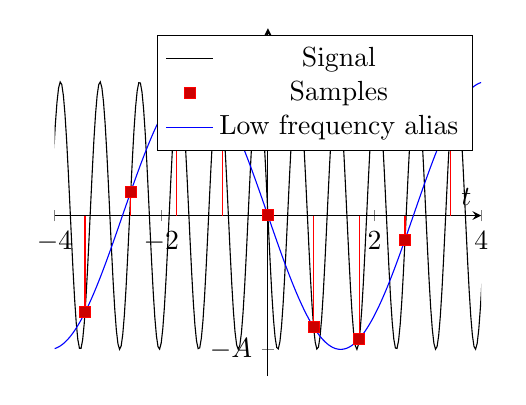
\begin{tikzpicture}
      \begin{axis}[domain=-6:6,
          width=7cm,height=6cm,ymin=-1.2,xmin=-4,ymax=1.4,xmax=4,
          ytick={-1,1},
          yticklabels={$-A$, $A$},
          xlabel=$t$, axis lines = center]
        \addplot[samples=400]{cos(deg(2.0*3.1415*1.35*x+3.14/2))};
        \addplot+[ycomb,samples=15]{cos(deg(2.0*3.1415*1.35*x+3.14/2))};
        \addplot[samples=400,color=blue]{cos(deg(2.0*3.1415*0.18333333333333335*x+3.14/2))};
        \node at (axis cs:0.9+0.45,1.1) [above, font={\footnotesize}]{$T_s$};
        \addplot[color=black] plot coordinates {(0.9,1.1) (2.0*0.9,1.1)};
        \legend{Signal,Samples,Low frequency alias}
      \end{axis}
    \end{tikzpicture}
    %\end{center}
    %The discrete-frequency spectrum of the signal is shown below:
    %\begin{center}
    \begin{tikzpicture}
      \begin{axis}[width=7cm,height=6cm,ymin=0,xmin=-4,ymax=1.5,xmax=4,  yticklabels={,,},
          xtick={-2,-1,1,2},
          xticklabels={$-2\pi$,$-\pi$,$\pi$,$2\pi$},
          xlabel=$\hat{\omega}$, axis lines = center]

        \addplot[ycomb,color=blue,mark=*,mark color=blue] plot coordinates {(2.2,1)};
        \addplot[ycomb,color=skyblue1,mark=*,mark color=skyblue] plot coordinates { (-1.8,1)};
        \addplot[ycomb,color=skyblue1,mark=*,mark color=skyblue] plot coordinates { (0.2,1)};

        \addplot[ycomb,color=red,mark=*,mark color=red] plot coordinates {(-2.2,1)};

        \addplot[ycomb,color=scarletred1,mark=*,mark color=scarletred1] plot coordinates {(1.8,1)};

        \addplot[ycomb,color=scarletred1,mark=*,mark color=scarletred1] plot coordinates {(-0.2,1)};

        \node at (axis cs:0.2,1.1) [below, rotate=90, font={\footnotesize}]{Alias};
        \node at (axis cs:-0.2,1.1) [above, rotate=90, font={\footnotesize}]{Alias};
        \node at (axis cs:1.8,1.1) [below, rotate=90, font={\footnotesize}]{Alias};
        \node at (axis cs:-1.8,1.1) [above, rotate=90, font={\footnotesize}]{Alias};

        \node at (axis cs:2.2,1.1) [below, rotate=90, font={\footnotesize}]{True};
        \node at (axis cs:-2.2,1.1) [above, rotate=90, font={\footnotesize}]{True};

        \draw [gray, thick] (axis cs:-1,0.0) rectangle (axis cs:1,1.4);
        %   \node at (axis cs:-0.4,1.1) [above, font={\footnotesize}]{$\frac{A}{2}e^{i\phi}$};
        %  \node at (axis cs:2.4,1.1) [above, font={\footnotesize}]{$\frac{A}{2}e^{-i\phi}$};
        % \node at (axis cs:-2.4,1.1) [above, font={\footnotesize}]{$\frac{A}{2}e^{i\phi}$};
      \end{axis}
    \end{tikzpicture}
  \end{center}
  \caption{Undersampling $f_s < f_0$. When the sample rate is smaller than the frequency of the 
  sinusoid there is less than one sample per sinusoid cycle. The discrete-time frequency 
  $\hat{\omega}>2\pi$ and a low-frequency alias of the high frequency sinusoid exists 
  in the principal spectrum.}
  \label{fig:undersampling}
\end{marginfigure}

\subsection{Nyquist oversampling criterion}
Let us assume that our continuous-time signal has non-zero spectral components with 
frequencies only within the range $|f|<\frac{1}{2}f_s$. This means that it has a 
Fourier transform representation of the form:
\begin{equation}
  x(t) = \frac{1}{2\pi}\int_{-\pi f_s}^{\pi f_s} \hat{x}(\omega)
  e^{i\omega t}d\omega\,\,.
\end{equation}
When such a signal is discretized, all the discrete-time spectral components of the 
signal land on the principal spectrum between $-\pi <\hat{\omega} < \pi$.

The band limited nature of the continuous-time signal also guarantees that no high frequency 
components will have low frequency aliases in the principal spectrum.
In this case, one can be certain that there is a one-to-one mapping between discrete-time 
frequency and continuous-time frequency. And therefore, no information is lost when discretizing the signal. 
In this case, the signal is said to be \emph{\index{oversampled}{oversampled}}.

To avoid aliasing of spectral component frequencies $f>f_s/2$ into the principal spectrum, 
the sample rate $f_s$ has to be at least twice the frequency of the highest frequency 
component of the signal:
\begin{equation}
  \boxed{
    f_s > 2f_{\mathrm{max}}
  }\,\,.
\end{equation}
It can be also expressed as
\begin{equation}
  \boxed{
    f_{\mathrm{max}}<\frac{1}{2}f_s
  }\,\,.
\end{equation}
This is called the \emph{\index{Nyquist oversampling}{Nyquist oversampling}} criterion. 
It is a special case of the more general Shannon-Nyquist sampling theorem.
If this criterion is not satisfied, then the signal is said to be \emph{undersampled}.

When deriving the Shannon-Nyquist sampling theorem, we will see that it is in some cases 
possible to retain information even when the signal is undersampled. 
Undersampling is a technique that is often used for sampling radio signals.

\newthought{For example}, the Nyquist frequency $f_{\mathrm{max}}$ of a real-valued 
signal sampled at $f_s=44.1$ kHz is $f_{\mathrm{max}}=22.05$ kHz. 
The sample rate 44.1 kHz is often used when digitizing audio, because audio signals 
within the human hearing range are between $0<f<20$ kHz and signals conveying audio 
signals only contain spectral components within this range.

\subsection{Nyquist zones}
\begin{marginfigure}
  \begin{center}
    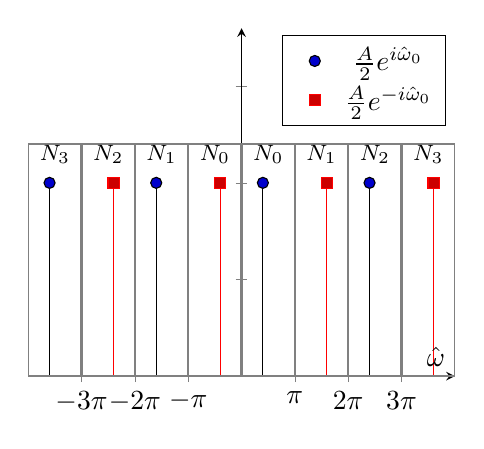
\begin{tikzpicture}
      \begin{axis}[width=7cm,height=6cm,ymin=0,xmin=-4,ymax=1.8,xmax=4,  yticklabels={,,},
          xtick={-3,-2,-1,0,1,2,3},
          xticklabels={$-3\pi$,$-2\pi$,$-\pi$,0,$\pi$,$2\pi$,$3\pi$},
          xlabel=$\hat{\omega}$, axis lines = center]
        \addplot+[ycomb,black] plot coordinates {(0.4,1) (2.4,1) (-1.6,1) (-3.6,1)};
        \addplot+[ycomb,red] plot coordinates {(-0.4,1) (1.6,1) (-2.4,1) (3.6,1)};
        \legend{$\frac{A}{2}e^{i\hat{\omega}_{0}}$,$\frac{A}{2}e^{-i\hat{\omega}_{0}}$};
        \draw [gray, thick] (axis cs:0,0.0) rectangle (axis cs:1,1.2);
        \draw [gray, thick] (axis cs:1,0.0) rectangle (axis cs:2,1.2);
        \draw [gray, thick] (axis cs:2,0.0) rectangle (axis cs:3,1.2);
        \draw [gray, thick] (axis cs:3,0.0) rectangle (axis cs:4,1.2);
        \draw [gray, thick] (axis cs:4,0.0) rectangle (axis cs:5,1.2);
        \draw [gray, thick] (axis cs:-1,0.0) rectangle (axis cs:0,1.2);
        \draw [gray, thick] (axis cs:-2,0.0) rectangle (axis cs:-1,1.2);
        \draw [gray, thick] (axis cs:-3,0.0) rectangle (axis cs:-2,1.2);
        \draw [gray, thick] (axis cs:-4,0.0) rectangle (axis cs:-3,1.2);
        \draw [gray, thick] (axis cs:-5,0.0) rectangle (axis cs:-4,1.2);
        \node at (axis cs:0.5,1.05) [above, font={\footnotesize}]{$N_0$};
        \node at (axis cs:1.5,1.05) [above, font={\footnotesize}]{$N_1$};
        \node at (axis cs:2.5,1.05) [above, font={\footnotesize}]{$N_2$};
        \node at (axis cs:3.5,1.05) [above, font={\footnotesize}]{$N_3$};
        \node at (axis cs:4.5,1.05) [above, font={\footnotesize}]{$N_4$};
        \node at (axis cs:-0.5,1.05) [above, font={\footnotesize}]{$N_0$};
        \node at (axis cs:-1.5,1.05) [above, font={\footnotesize}]{$N_1$};
        \node at (axis cs:-2.5,1.05) [above, font={\footnotesize}]{$N_2$};
        \node at (axis cs:-3.5,1.05) [above, font={\footnotesize}]{$N_3$};
        \node at (axis cs:-4.5,1.05) [above, font={\footnotesize}]{$N_4$};
      \end{axis}
    \end{tikzpicture}
  \end{center}
  \caption{Nyquist zones.}
  \label{fig:nyq_zones}
\end{marginfigure}

If spectral components of a real-valued continuous-time signal are only located 
between $k f_s/2\le|f|<(k+1)f_s/2$ for only one value of $k$ and if there are no 
non-zero spectral components elsewhere, then one can still recover the 
continuous-time signal from the discrete-time representation of the signal,
using the a priori information that the signals are within this range of frequencies. 
This is the more general sampling criterion for real-valued signals.

These regions, which are shown in Figure \ref{fig:nyq_zones}, are called Nyquist zones. 
In each of these cases, all the low frequency aliases of the signal will be confined
with the principal spectrum $\pm \pi$. Because no signals from outside the specific 
Nyquist zone are present, there is no chance of two continuous-time spectral
components mapping to the same normalized angular frequency within the principal spectrum.

\begin{marginfigure}
  \begin{center}
    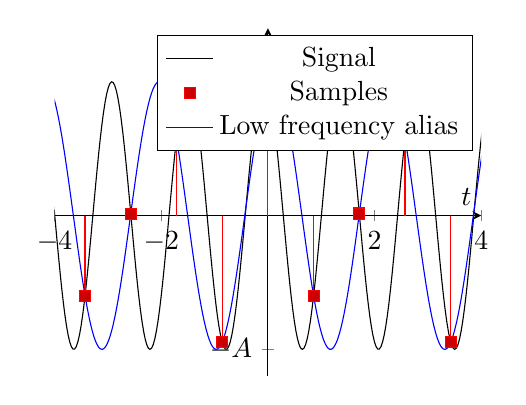
\begin{tikzpicture}
      \begin{axis}[domain=-6:6,
          width=7cm,height=6cm,ymin=-1.2,xmin=-4,ymax=1.4,xmax=4,
          ytick={-1,1},
          yticklabels={$-A$, $A$},
          xlabel=$t$, axis lines = center]
        \addplot[samples=400]{cos(deg(2.0*3.1415*0.7*x+0.3))};
        \addplot+[ycomb,samples=15]{cos(deg(2.0*3.1415*0.7*x+0.3))};
        \addplot[samples=400,color=blue]{cos(deg(2.0*3.1415*0.4666666666666667*x-0.3))};
        \node at (axis cs:0.9+0.45,1.1) [above, font={\footnotesize}]{$T_s$};
        \addplot plot coordinates {(0.9,1.1) (2.0*0.9,1.1)};
        \legend{Signal,Samples,Low frequency alias}
      \end{axis}
    \end{tikzpicture}
  \end{center}

  \begin{center}
    \begin{tikzpicture}
      \begin{axis}[width=7cm,height=6cm,ymin=0,xmin=-4,ymax=1.5,xmax=4,  yticklabels={,,},
          xtick={-2,-1,1,2},
          xticklabels={$-2\pi$,$-\pi$,$\pi$,$2\pi$},
          xlabel=$\hat{\omega}$, axis lines = center]

        \addplot[ycomb,color=blue,mark=*,mark color=blue] plot coordinates {((-1.8,1)};
        \addplot[ycomb,color=skyblue1,mark=*,mark color=skyblue] plot coordinates { (2.2,1)};
        \addplot[ycomb,color=skyblue1,mark=*,mark color=skyblue] plot coordinates { (0.2,1)};

        \addplot[ycomb,color=red,mark=*,mark color=red] plot coordinates {(1.8,1)};

        \addplot[ycomb,color=scarletred1,mark=*,mark color=scarletred1] plot coordinates {(-2.2,1)};

        \addplot[ycomb,color=scarletred1,mark=*,mark color=scarletred1] plot coordinates {(-0.2,1)};

        \node at (axis cs:0.2,1.1) [below, rotate=90, font={\footnotesize}]{Alias};
        \node at (axis cs:-0.2,1.1) [above, rotate=90, font={\footnotesize}]{Alias};
        \node at (axis cs:1.8,1.1) [below, rotate=90, font={\footnotesize}]{True};
        \node at (axis cs:-1.8,1.1) [above, rotate=90, font={\footnotesize}]{True};

        \node at (axis cs:2.2,1.1) [below, rotate=90, font={\footnotesize}]{Alias};
        \node at (axis cs:-2.2,1.1) [above, rotate=90, font={\footnotesize}]{Alias};

        \draw [gray, thick] (axis cs:-1,0.0) rectangle (axis cs:1,1.4);
        %   \node at (axis cs:-0.4,1.1) [above, font={\footnotesize}]{$\frac{A}{2}e^{i\phi}$};
        %  \node at (axis cs:2.4,1.1) [above, font={\footnotesize}]{$\frac{A}{2}e^{-i\phi}$};
        % \node at (axis cs:-2.4,1.1) [above, font={\footnotesize}]{$\frac{A}{2}e^{i\phi}$};
      \end{axis}
    \end{tikzpicture}
  \end{center}
  \caption{Folded undersampling $f_{0} < f_s < 2 f_0$, There are between 1 and 2 samples for each cycle of the continuous-time sinusoid. The low frequency alias is phase flipped.}
  \label{fig:folded_undersampling}
\end{marginfigure}

When $k=0$, this case is called an \emph{oversampled} signal. This is the special case that 
the Nyquist oversampling criterion applies to. When $k = 1$, the signal sampling is 
called \emph{folded undersampled} signal. In this case, the aliased signal 
in the principal spectrum is flipped in frequency and phase relative to the 
continuous-time spectrum. When $k=2$, the signal is \emph{undersampled}. 
These different cases are shown in Figures \ref{fig:oversampling}, 
\ref{fig:folded_undersampling}, and \ref{fig:undersampling}.

There are many cases, especially with modern software defined radios, 
where undersampling or folded undersampling at Nyquist zones $k>0$ are used. 
This violates the simple $f_s > 0.5 f_{\mathrm{max}}$ Nyquist oversampling criterion, 
but is still perfectly fine, as long as the original continuous-time signal has 
spectral components confined within a Nyquist zone.


\subsection{Complex-valued signals}
For complex-valued signals, the \emph{principal spectrum} is the same as it is for 
real-valued signals. In discrete-time angular frequency it is $-\pi<\hat{\omega}<\pi$ and 
in continuous-time frequency $-\frac{1}{2}f_s<f<\frac{1}{2}f_s$. However, because there 
are no conjugate symmetric negative frequency pairs, both negative and positive frequencies 
can be used in this frequency band. Therefore, the effective bandwidth is twice that of 
real-valued signals sampled at the sample rate $f_s$, as both positive and negative 
frequency components can be used independently to encode information.

To ensure a one-to-one relationship between the discrete-time signal and the 
continuous-time signal, the sample rate $f_s$ has to be at least the difference 
between the largest and smallest frequency component
\begin{equation}
  \boxed{
  f_s > f_{\mathrm{max}}-f_{\mathrm{min}}
  }\,\,.
\end{equation}
if the frequency domain representation of the complex-valued signal is within a 
continuous range of frequencies between $f_{\mathrm{min}}$ and $f_{\mathrm{max}}$. 
This avoids having two continuous-time spectral components with different frequencies 
aliasing onto the same discrete-time frequency within the principal 
spectrum\sidenote{The most general sampling criterion involves investigating 
the relationship between the frequency domain representation of the 
continuous-time signal and the frequency domain representation of the 
discretized signal, which we will discuss later when deriving the Shannon sampling theorem.}.
This is another form of the Shannon-Nyquist sampling criterion, 
which applies only to complex-valued signals.

Figure \ref{fig:complex_aliasing} below illustrates aliasing with complex sinusoidal signals. 
Here, a complex sinusoidal signal with frequency $1.2\frac{f_s}{2}$ that is sampled with 
frequency $f_s$ aliases to $-0.8\frac{f_s}{2}$ in the principal spectrum.

\begin{marginfigure}
  \begin{center}
    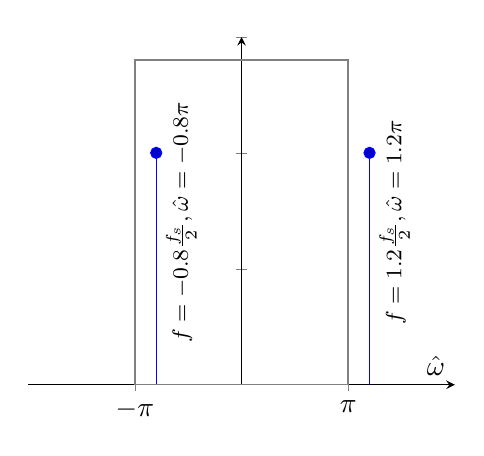
\begin{tikzpicture}
      \begin{axis}[width=7cm,height=6cm,ymin=0,xmin=-2,ymax=1.5,xmax=2,  yticklabels={,,},
          xtick={-1,1},
          xticklabels={$-\pi$,$\pi$},
          xlabel=$\hat{\omega}$, axis lines = center]
        \addplot+[ycomb] plot coordinates {((-0.8,1) (1.2,1)};
        %    \addplot+[ycomb] plot coordinates {(-1.2,1) (0.8,1)};
        \node at (axis cs:1.2,0.7) [below, rotate=90, font={\footnotesize}]{$f=1.2\frac{f_s}{2}, \hat{\omega}=1.2\pi$};
        \node at (axis cs:-0.8,0.7) [below, rotate=90, font={\footnotesize}]{$f=-0.8\frac{f_s}{2}, \hat{\omega}=-0.8\pi$};
        \draw [gray, thick] (axis cs:-1,0.0) rectangle (axis cs:1,1.4);

        %   \node at (axis cs:-0.4,1.1) [above, font={\footnotesize}]{$\frac{A}{2}e^{i\phi}$};
        %  \node at (axis cs:2.4,1.1) [above, font={\footnotesize}]{$\frac{A}{2}e^{-i\phi}$};
        % \node at (axis cs:-2.4,1.1) [above, font={\footnotesize}]{$\frac{A}{2}e^{i\phi}$};
      \end{axis}
    \end{tikzpicture}
  \end{center}
  \caption{Aliasing of a complex sinusoidal spectral component into the principal spectrum. No conjugate symmetric negative frequency spectral components complicate the aliasing of the signal into the principal spectrum.}
  \label{fig:complex_aliasing}
\end{marginfigure}

\newthought{An example of aliasing of two complex sinusoidal signals} is shown below. 
If a continuous-time signal consists of two complex sinusoidal signals:
\begin{equation}
  z(t)=a_1 e^{i 2\pi f_1 t} + a_2 e^{i 2\pi f_2 t}\,\,,
\end{equation}
with frequencies $f_1= 1.2 f_s/2$ and $f_2=0.8 f_s/2$.

When this signal is sampled with a sample-rate of $f_s$, the Nyquist oversampling criterion 
for real-valued signals is violated, because $f_1 > f_s/2$.
However, this is a complex-valued signal, and we only need $f_{\mathrm{max}} - f_{\mathrm{min}} < f_s$ 
to hold in the more general case for complex-valued signals.

This condition is not violated. To see that everything is fine, we
translate both of the sinusoidal signals into the principal spectrum:
\begin{align}
  z[n] & = a_1 e^{i 1.2\pi n }+ a_2 e^{i 0.8\pi n }       \\
       & = a_1 e^{-i 0.8\pi n }+ a_2 e^{i 0.8\pi n }\,\,.
\end{align}
We see that the signals land at $\hat{\omega} = \pm 0.8\pi$ in the
principal spectrum. The two spectral components are distinct, and if we have sufficient information 
about the lowest and highest frequency component of the signal 
(i.e., we know $f_{\mathrm{min}}$ and $f_{\mathrm{max}}$), 
we can still perfectly reconstruct the signal.

\if 0
  For example, if we knew that $f_{\mathrm{min}} = 0$ and $f_{\mathrm{max}} = f_s$, 
  we would know that all spectral components with discrete-time angular frequencies in 
  the principal spectrum between $-\pi$ and $0$ would correspond to continuous-time frequencies 
  between $f_s/2$ and $f_s$. Similarly, we would know that all spectral components with 
  discrete-time angular frequencies between 0 and $\pi$ in the principal spectrum would be 
  mapped to continuous-time frequencies between 0 and $f_s/2$.
\fi

\subsection{2D aliasing}
Consider a two-dimensional signal $I(x,y) \in \mathbb{R}$, which is discretized as follows:

\begin{equation}
  I[n,m]=I(n T_x, m T_y)\,\,.
\end{equation}
Here $T_x$ and $T_y$ are sample spacing in the $x$ and $y$ direction, and $n$, and $m$ are sample 
indices in the two dimensions.

A 2D signal has a spectral representation, which is given by 2D complex exponential signals:
\begin{equation}
  I(x,y) = \frac{1}{(2\pi)^{2}} \int_{-\infty}^{\infty} \int_{-\infty}^{\infty} \hat{I}(\omega_1,\omega_2) e^{i(\omega_1 x + \omega_2 y)} d\omega_1 d\omega_2\,\,.
\end{equation}
\begin{marginfigure}
  \begin{center}
    \includegraphics[width=\textwidth]{ch09/figures/briko.jpg}
    \includegraphics[width=\textwidth]{ch09/figures/brickd.jpg}
  \end{center}
  \caption{Example of aliasing behavior in a 2D image. Above: original, Below: aliased. When scaling an image (reducing its size),
    it is important to apply an anti-aliasing filter that removes high frequency spectral components from the
    high resolution image before it is scaled down to a lower resolution. Otherwise, there is a risk that 
    high frequency periodic structures
    will appear as low frequency structures in the scaled image, as shown in the lower image.
    Anti-aliasing filtering is a standard feature of most image processing libraries, and one rarely 
    sees the type of aliasing shown in the bottom figure in practice.}
  \label{fig:brick_alias}
\end{marginfigure}
To study aliasing behavior in 2D, it is sufficient to study aliasing effects on individual spectral components:
\begin{equation}
  z(x,y) = a e^{i (\omega_1 x + \omega_2 y) }\,\,,
\end{equation}
When discretizing the 2D complex exponential spectral component, one can obtain aliasing behavior 
when sampling through $2\pi$-periodicity:
\begin{align}
  z[n,m] & = a e^{i(\omega_1 T_x n + \omega_2 T_y m ) }                                \\
         & =a e^{i([\omega_1 T_x + 2\pi k]n + [\omega_2 T_y + 2\pi \ell]m)}            \\
         & =a e^{i([\hat{\omega}_1 + 2\pi k]n + [\hat{\omega}_{2} + 2\pi \ell]m)}\,\,.
\end{align}
Here $k,l \in \mathbb{Z}$.

Figure \ref{fig:brick_alias} demonstrates aliasing in 2D. This is
discretized in such a way that the high spatial frequency brick
pattern on the side of the building becomes undersampled, and a low
frequency alias is seen.

\if 0 
\subsection{Reconstruction}
\begin{marginfigure}
  \tikzstyle{int}=[draw, minimum size=2em]
  \tikzstyle{init} = [pin edge={to-,thin,black}]
  \begin{center}
    %  \resizebox{\columnwidth}{!}{%
    \begin{tikzpicture}[every text node part/.style={align=center},node distance=3cm,auto,>=latex']
      \node [int] (a) {D-to-C \\ $T_s$};
      \node (b) [left of=a,node distance=2cm, coordinate] {a};
      %    \node (c) [below=a,node distance=3cm] {a};

      %\node [int, pin={[init]above:$p_0$}] (c) [right of=a] {$\frac{1}{s}$};
      \node [coordinate] (end) [right of=a, node distance=3cm]{};
      \path[->] (b) edge node {$x[n]$} (a);
      \draw[->] (a) edge node {$x(t)$} (end) ;
    \end{tikzpicture}
    % }
  \end{center}
  \caption{A Discrete-time to Continuous-time (D-to-C) converter.}
\end{marginfigure}

Reconstruction involves transforming a discrete-time signal into a continuous-time signal. 
This type of operation is done, e.g., when
translating an audio signal into air pressure variations to create sound.

In order to convert a discrete-time signal into a continuous-time signal, some form 
of interpolation is needed in order to fill in the space between the samples. 
This is the function of a reconstruction filter, or a discrete-time to continuous-time (D-to-C) system:
\begin{equation}
  x(t) = \mathcal{R}\{x[n]\}\,\,.
\end{equation}
The ingredients that are needed to reconstruct the signal are the samples $x[n]$, information about the
sampling rate $T_s=1/f_s$, and information about the Nyquist zone that the signal is within.

This is equivalent to knowing the true values of the discrete-time frequencies $\hat{\omega}$ of all the discretized spectral
components, i.e., being able to rule out all the aliases using a priori knowledge of the frequency band that the signal lies in.

There are several ways to perform this reconstruction. If the analytical form of the signal is 
known, as in the case of a sinusoid, the signal can be generated analytically based on the 
phase and amplitude of the signal. In other cases, some form of interpolation is needed.

\subsection{Interpolation filters}
In this section, we'll only cover reconstruction of oversampled signals\footnote{It is possible to derive interpolation filters
  for reconstruction of undersampled signals in the same way, but this is beyond the scope of this course.} that satisfy
the Nyquist-Shannon sampling criterion $f_s > 2f_{\mathrm{max}}$, i.e., 
the spectral components of the signal are between $-f_s/2 < f < f_s/2$.

We can convert a discrete-time signal into a continuous-time signal using an interpolation filter of the form:
\begin{equation}
  x(t) = \sum_{n=-\infty}^{\infty} x[n]p(t-nT_s)\,\,.
\end{equation}
Theoretically, this interpolation filter can use the discrete-time samples to obtain the continuous-time reconstruction.
\begin{marginfigure}
  \begin{center}
    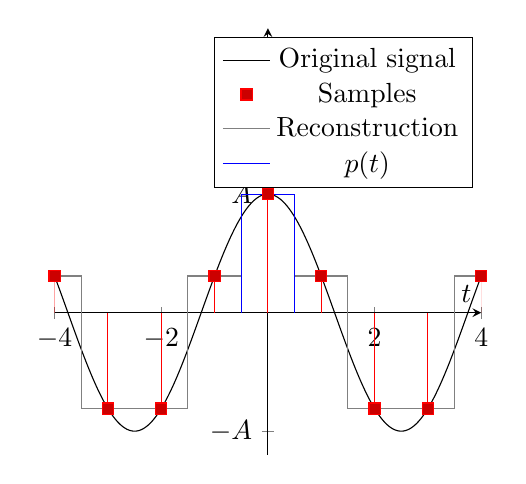
\begin{tikzpicture}
      \begin{axis}[domain=-5:5,
          width=7cm,height=7cm,ymin=-1.2,xmin=-4,ymax=2.4,xmax=4,
          ytick={-1,1},
          yticklabels={$-A$, $A$},
          xlabel=$t$, axis lines = center]
        \addplot[samples=400]{cos(deg(2.0*3.1415*0.2*x))};
        \addplot+[ycomb,samples=11]{cos(deg(2.0*3.1415*0.2*x))};
        \addplot[mark=none,color=gray] plot coordinates {(-4.5,0.30901699) (-3.5,0.30901699) (-3.5,-0.80901699) (-2.5,-0.80901699) (-2.5,-0.80901699) (-1.5,-0.80901699) (-1.5,0.30901699) (-0.5,0.30901699) (-0.5,1.) (0.5,1.) (0.5,0.30901699) (1.5,0.30901699) (1.5,-0.80901699) (2.5,-0.80901699) (2.5,-0.80901699) (3.5,-0.80901699)  (3.5,0.30901699) (4.5,0.30901699)};

        \addplot[mark=none,color=blue] plot coordinates {(-0.5,0.0) (-0.5,1.0) (0.5,1.0) (0.5,0)};                             %  \addplot[samples=100,domain=-0.5:0.5,color=blue]{1};

        \legend{Original signal,Samples, Reconstruction, $p(t)$}
      \end{axis}
    \end{tikzpicture}
  \end{center}
  \caption{Zero-order hold interpolation.}
  \label{fig:z-o-hold}
\end{marginfigure}

\newthought{The zero-order hold filter} is the simplest interpolation filter. 
It obtains a constant value for the duration of a sample.
The filter in this case has the following mathematical definition:
\begin{equation}
  p(t) = \left\{
  \begin{array}{rcr}
    1 & \mathrm{when}      & -\frac{T_s}{2} < t \le \frac{T_s}{2} \\
    0 & \mathrm{otherwise} &                                      \\
  \end{array}
  \right\} \,\,.
\end{equation}
The generated continuous-time signal looks like the one shown in Figure \ref{fig:z-o-hold}.

\begin{marginfigure}
  \begin{center}
    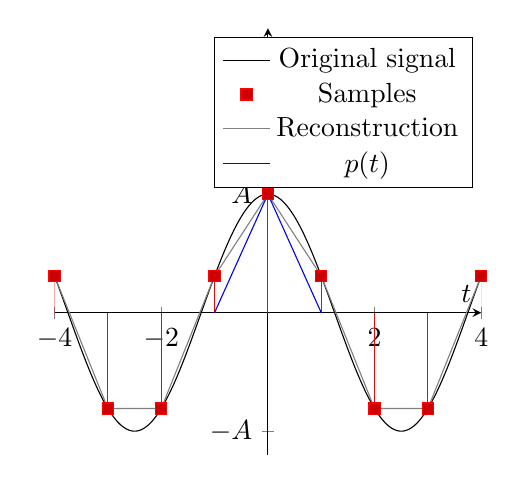
\begin{tikzpicture}
      \begin{axis}[domain=-5:5,
          width=7cm,height=7cm,ymin=-1.2,xmin=-4,ymax=2.4,xmax=4,
          ytick={-1,1},
          yticklabels={$-A$, $A$},
          xlabel=$t$, axis lines = center]
        \addplot[samples=400]{cos(deg(2.0*3.1415*0.2*x))};
        \addplot+[ycomb,samples=11]{cos(deg(2.0*3.1415*0.2*x))};
        \addplot[mark=none,color=gray] plot coordinates {(-4,0.30901699) (-3,-0.80901699) (-2,-0.80901699) (-1,0.30901699) (0.0,1.)  (1,0.30901699) (2,-0.80901699) (3,-0.80901699) (4,0.30901699) };
        \addplot[samples=100,domain=-1:1,color=blue]{1-abs(x)};

        \legend{Original signal,Samples, Reconstruction, $p(t)$}
      \end{axis}
    \end{tikzpicture}
  \end{center}
  \caption{Linear interpolation filter.}
  \label{fig:lin_int_filter}
\end{marginfigure}

The zero-order hold filter only needs one sample at a time. However, the continuous-time signal has large steps.
The zero-order hold filter approaches the continuous-time signal only when $T_s\rightarrow 0$ -- i.e., 
when the sample rate is infinitely large.

\newthought{A Linear interpolation filter} is defined as follows:
\begin{equation}
  p(t) = \left\{
  \begin{array}{rcr}
    1-\frac{|t|}{T_s} & \mathrm{when}      & -T_s < t < T_s \\
    0                 & \mathrm{otherwise} &                \\
  \end{array}
  \right\} \,\,.
\end{equation}
It applies a linear interpolation between two consecutive samples. The generated continuous-time signal 
is depicted in Figure \ref{fig:lin_int_filter}.

\newthought{The ideal reconstruction filter} is based on the
Shannon-Nyquist sampling theorem. It guarantees theoretically that a continuous-time real-valued signal 
can be perfectly reconstructed from discrete-time samples for
signals occupying the band $-f_s/2 < f < f_s/2$, if $f_s > 2f_{\mathrm{max}}$.
Here $f_{\mathrm{max}}$ is the maximum frequency component within the signal. We'll prove this 
theorem at the end of this chapter.

In order to reconstruct the signal perfectly in a mathematical sense, an ideal 
reconstruction filter must be used.
Something approximately resembling a truncated or tapered version of an ideal reconstruction filter is 
typically used in real world applications.

The form of this ideal reconstruction filter can be derived from the inverse Fourier transform of a 
rectangular shaped window that in frequency domain is an ideal low pass filter:
\begin{equation}
  P(\omega) = \left\{
  \begin{array}{rcr}
    T_s & \mathrm{when}      & |\omega| \le \pi f_s \\
    0   & \mathrm{otherwise} &                      \\
  \end{array}
  \right. \,\,.
\end{equation}
\begin{marginfigure}
  \begin{center}
    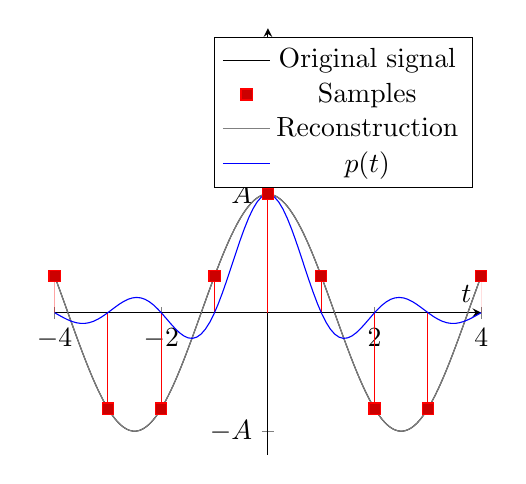
\begin{tikzpicture}
      \begin{axis}[domain=-5:5,
          width=7cm,height=7cm,ymin=-1.2,xmin=-4,ymax=2.4,xmax=4,
          ytick={-1,1},
          yticklabels={$-A$, $A$},
          xlabel=$t$, axis lines = center]
        \addplot[samples=400]{cos(deg(2.0*3.1415*0.2*x))};
        \addplot+[ycomb,samples=11]{cos(deg(2.0*3.1415*0.2*x))};
        \addplot[samples=400,mark=none,color=gray]{cos(deg(2.0*3.1415*0.2*x))};
        \addplot[samples=100,domain=-4:4,color=blue]{sin(deg((3.14)*(x+0.0000001)))/(3.14*(x+0.000001))};

        \legend{Original signal,Samples, Reconstruction,$p(t)$}
      \end{axis}
    \end{tikzpicture}
  \end{center}
  \caption{Ideal reconstruction filter.}
\end{marginfigure}
Here $P(\omega)$ is the Fourier transform of the reconstruction
filter, $\omega$ is angular frequency. The resulting ``ideal''
reconstruction filter is:
\begin{align}
  p(t) & =\frac{1}{2\pi}\int_{-\infty}^{\infty} P(\omega)e^{i\omega t}d\omega \\
       & = \frac{T_s}{\pi t}\sin\left(\frac{\pi}{T_s}t\right)\,\,.
\end{align}
This filter is infinitely long, which implies that all samples need to be used in order for the 
reconstructed signal to be mathematically perfect.
\fi

\if 0
  Similar reconstruction filters exists for other Nyquist zones, which allow perfect 
  reconstruction of undersampled signals, which satisfy the Shannon-Nyquist sampling criterion. 
  Such filters use ideal reconstruction filters that can be derived from idealized band-pass filters:
  \begin{equation}
    P(\omega) = \left\{
    \begin{array}{rcr}
      T_s & \mathrm{when}      & k\omega_s/2 \le |\omega| < (k+1)\omega_s/2 \\
      0   & \mathrm{otherwise} &                                            \\
    \end{array}
    \right\} \,\,.
  \end{equation}
  Here $k$ specifies the Nyquist zone for which the signal is to be reconstructed in.
\fi

\section{Shannon's sampling theorem}
\begin{marginfigure}
  \begin{center}
    \includegraphics[width=\textwidth]{ch09/figures/shannon_mouse.png}
  \end{center}
  \caption{Claude Elwood Shannon. Photo: Bell Labs.}
\end{marginfigure}

Shannon's sampling theorem is a fundamental theorem in information theory and signal 
processing\sidenote{This theorem was discovered by Edmund Whittaker 33 years before Claude Shannon, 
and thus sometimes the sampling theory is called the Whittaker-Shannon sampling theorem.\cite{whittaker1915xviii,shannon1948mathematical}}. 
It relates the sample-rate of a discrete-time signal to the bandwidth of a continuous-time signal in frequency domain.
The full form of the theory is not just: ``use a sample-rate that is at least twice as large as the largest 
frequency component in the continuous-time signal''. There are other solutions, which also guarantee that no 
information about the signal is lost.
The most general way to investigate if information is lost when discretizing a signal is to explore 
the relationship between the Fourier transform of the signal, and the Fourier transform of the discretized signal.

We will assume that information is contained in the shape of the signal $x(t)$. 
This signal is assumed to be band-limited in frequency domain.
This means that the spectrum is zero valued outside a certain range of frequencies: 
$\hat{x}(\omega) = 0$ when $\omega < \omega_{\mathrm{min}}$ or $\omega > \omega_{\mathrm{max}}$.

Is it possible to form a discrete-time signal $x[n]$ from $x(t)$ in such a way that $x[n]$ contains sufficient information to
allow us to perfectly reconstruct $x(t)$? In other words, can we perfectly reconstruct a continuous-time signal $x(t)$ from
its discrete-time representation? This is the question that Shannon studied, and his sampling theorem provides an answer to.

\subsection{Sampling}
\begin{marginfigure}[3cm]
  \begin{center}
    \includegraphics[width=\textwidth]{ch09/figures/whittaker.jpg}
  \end{center}
  \caption{Sir Eduard Whittaker. Photo: National Portrait Gallery.}
\end{marginfigure}

In the idealized case, sampling of a signal is selection of samples from a continuous-time signal:
\begin{equation}
  x[n] = x(nT_s)
\end{equation}
where $T_s$ is the sample spacing. This is the inverse of the sample-rate $T_s = f_s^{-1}$. 
We can express this sampling process using the Dirac delta function, 
where a delayed Dirac delta ``samples'' the value of the signal $x(t)$ at time $nT_s$:
\begin{equation}
  x[n] = \int_{-\infty}^{\infty}x(t)\delta(t-nT_s)dt = x(nT_s).
\end{equation}
We can use a train of Dirac delta functions (Dirac comb)
\begin{equation}
  s(t) = \sum_{n=-\infty}^{\infty}\delta(t-nT_s),
\end{equation}
to represent the sampled signal in continuous-time:
\begin{align}
  x_s(t) & = x(t) s(t)                                     \\
         & = x(t) \sum_{n=-\infty}^{\infty} \delta(t-nT_s) \\
         & = \sum_{n=-\infty}^{\infty} x[n]\delta(t-nT_s)
\end{align}
The sampled signal $x_s(t)$ is a continuous-time signal, which has the same information 
content as the array of samples $x[n]$. This means that $x_s(t)$ can be formed just by 
knowledge of the discrete-time signal $x[n]$.

\subsection{Fourier series representation for Dirac comb}
The Dirac comb
\begin{equation}
  s(t) = \sum_{k=-\infty}^{\infty} \delta(t-kT_s),
\end{equation}
is a periodic function with period $T_s$. Therefore, it is possible to express it as a Fourier series:
\begin{equation}
  s(t) = \sum_{k=-\infty}^{\infty} c_k e^{i\frac{2\pi}{T_s}kt}.
\end{equation}
The coefficients of the Fourier series can be obtained using the Fourier series synthesis equation, 
by integrating over one period of the function:
\begin{align}
  c_k & = \frac{1}{T_s}\int_{-T_s/2}^{T_s/2} \left[\sum_{n=-\infty}^{\infty} \delta(t-nT_s) \right] e^{-i\frac{2\pi}{T_s}kt}dt \\
      & =\frac{1}{T_s}\int_{-T_s/2}^{T_s/2} \delta(t)  e^{-i\frac{2\pi}{T_s}kt}dt                                              \\
      & =\frac{1}{T_s}e^{-i\cdot 0}                                                                                            \\
      & =\frac{1}{T_s}
\end{align}
We also note that $2\pi/T_s = \omega_s$, which is the sample-rate expressed as an angular frequency. 
The Fourier series representation of the Dirac-comb is therefore:
\begin{equation}
  s(t) = \frac{1}{T_s}\sum_{k=-\infty}^{\infty} e^{i k \omega_s t}.
\end{equation}
This Fourier series representation can now be substituted to represent the sampling operation as:
\begin{align}
  x_s(t) & = x(t)s(t)                                                                     \\
         & = x(t)  \left(\frac{1}{T_s}\sum_{k=-\infty}^{\infty} e^{i k \omega_s t}\right)
\end{align}

\subsection{Spectral representation of $x_s(t)$ and $x(t)$}
We then Fourier transform $x_s(t)$ to study the relationship between the sample-rate and 
the bandwidth of the signal.
We use the property that multiplication in time domain is convolution in frequency domain. 
The Fourier transform of $x(t)$ is $\hat{x}(\omega)$.
The Fourier transform of $s(t)$ is $\hat{s}(\omega)$. We also make use of the fact that the 
Fourier transform of $e^{i k \omega_s t}$ is $2\pi\delta(\omega-k\omega_s)$:
\begin{align}
  \hat{x}_s(\omega) & = \frac{1}{2\pi}  \hat{x}(\omega)*\hat{s}(\omega)\label{eq:xs_spec}                                                                                            \\
                    & = \frac{1}{2\pi}\int_{-\infty}^{\infty}\hat{x}(\omega') \hat{s}(\omega-\omega')d\omega'                                                                        \\
                    & = \frac{1}{2\pi} \int_{-\infty}^{\infty} \hat{x}(\omega')\left(\frac{1}{T_s}\sum_{k=-\infty}^{\infty} 2\pi \delta(\omega- k\omega_s - \omega')\right) d\omega' \\
                    & = \frac{1}{T_s} \sum_{k=-\infty}^{\infty}\int_{-\infty}^{\infty} \hat{x}(\omega')\delta(\omega - k\omega_s - \omega') d\omega'                                 \\
                    & = \frac{1}{T_s} \sum_{k=-\infty}^{\infty} \hat{x}(\omega-k\omega_s).
\end{align}
In other words, the Fourier transform of the sampled function $x_s(t)$ is infinitely 
many copies of $\hat{x}(\omega)$, each shifted by $k\omega_s$ and scaled in 
amplitude by $\frac{1}{T_s}$.

We illustrate this using the following two figures. The first one depicts the magnitude 
spectrum of the original continuous-time signal $x(t)$:
\begin{center}
  \begin{tikzpicture}
    \begin{axis}[width=15cm,height=5cm,ymin=0,ymax=3,
        xmin=-11,xmax=11,
        xlabel={$\omega$},
        ylabel={$|\hat{x}(\omega)|$},
        axis x line=center,
        axis y line=center,
        yticklabels={,,,},
        xtick={-6,-3,3,6},
        xticklabels={$-\omega_s$,$-\omega_s/2$,$\omega_s/2$,$\omega_s$}
      ]
      \addplot[mark=none,color=blue] plot coordinates {(-10,0.0) (-1,0) (-0.8,2*0.8) (-0.2,2*1) (0,0) (0.2,2*1) (0.8,2*0.8) (1,0)  (7,0)};

    \end{axis}
  \end{tikzpicture}
\end{center}
The sampled signal $x_s(t)$ has a periodic spectrum $\hat{x}_s(\omega)
  = \hat{x}_s(\omega+k\omega_s)$, which has a period $\omega_s$:
\begin{center}
  \begin{tikzpicture}
    \begin{axis}[width=15cm,height=5cm,ymin=0,ymax=3,
        xmin=-11,xmax=11,
        xlabel={$\omega$},
        ylabel={$|\hat{x}_s(\omega)|$},
        axis x line=center,
        axis y line=center,
        yticklabels={,,,},
        xtick={-6,-3,3,6},
        xticklabels={$-\omega_s$,$-\omega_s/2$,$\omega_s/2$,$\omega_s$}
      ]
      \addplot[mark=none,color=blue] plot coordinates {(-10,0.0) (-7,0) (-6.8,2*0.8) (-6.2,2*1) (-6,0) (-5.8,2*1) (-5.2,2*0.8) (-5,0) (-1,0) (-0.8,2*0.8) (-0.2,2*1) (0,0) (0.2,2*1) (0.8,2*0.8) (1,0)  (5,0) (5.2,2*0.8) (5.8,2*1) (6,0) (6.2,2*1) (6.8,2*0.8) (7,0)};
      \draw node at (axis cs:-9,0.5) {$\cdots$};
      \draw node at (axis cs:9,0.5) {$\cdots$};
    \end{axis}
  \end{tikzpicture}
\end{center}
This probably already provides some idea of what the sample-rate should be, in order to 
avoid losing information. The most straightforward answer is that if the spectrum of the 
original signal $\hat{x}(\omega)$ is confined within the limits of $\pm \omega_s/2$, 
then no overlap between the different copies of $\hat{x}(\omega)$ occurs.

There are other solutions that avoid aliasing for real-valued signals. The original 
signal $\hat{x}(\omega)$ might also be confined in frequency to one of 
the intervals $n \omega_s/2 \le |\omega| < (n+1)\omega_s/2$ with $n\in\mathbb{Z}$.
This property is widely used when sampling radio signals that are at a much higher 
frequency than the sample rate. This type of sampling strategy is called undersampling.

\subsection{Aliasing}
If the different copies of $\hat{x}(\omega)$ in $\hat{x}_s(\omega)$ overlap, then 
aliasing occurs. For example, if the spectrum of $\hat{x}(\omega)$ extends over the 
limits $\pm \omega_s/2$, then there are regions where $\hat{x}_s(\omega)$ is occupied 
by two or more spectral components of $\hat{x}(\omega)$ at the same time.

If the frequency extent of the original signal $\hat{x}(\omega)$ is larger than $\omega_s$, 
then aliasing occurs as shown below:
\begin{center}
  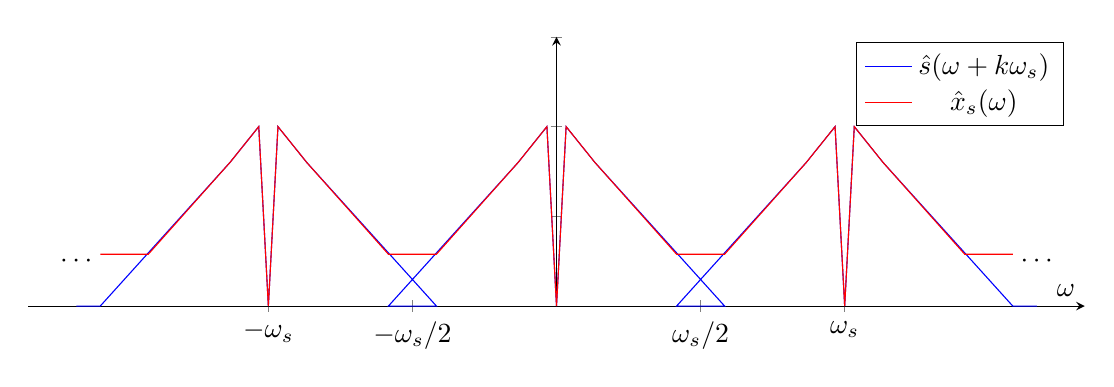
\begin{tikzpicture}
    \begin{axis}[width=15cm,height=5cm,ymin=0,ymax=3,
        xmin=-11,xmax=11,
        xlabel={$\omega$},
        ylabel={},
        axis x line=center,
        axis y line=center,
        yticklabels={,,,},
        xtick={-6,-3,3,6},
        xticklabels={$-\omega_s$,$-\omega_s/2$,$\omega_s/2$,$\omega_s$}
      ]
      \addplot[mark=none,color=blue] plot coordinates {(-10,0.0) (-9.5,0) (-6.8,2*0.8) (-6.2,2*1) (-6,0) (-5.8,2*1) (-5.2,2*0.8) (-2.5,0) (-3.5,0) (-0.8,2*0.8) (-0.2,2*1) (0,0) (0.2,2*1) (0.8,2*0.8) (3.5,0)  (2.5,0) (5.2,2*0.8) (5.8,2*1) (6,0) (6.2,2*1) (6.8,2*0.8) (9.5,0) (10,0) } ;
      \addlegendentry{$\hat{s}(\omega + k\omega_s)$}
      \addplot[mark=none,color=red] plot coordinates {(-9.5,0.5775) (-8.5,0.5775) (-6.8,2*0.8) (-6.2,2*1) (-6,0) (-5.8,2*1) (-5.2,2*0.8) (-3.5,0.5775) (-2.5,0.5775) (-0.8,2*0.8) (-0.2,2*1) (0,0) (0.2,2*1) (0.8,2*0.8) (2.5,0.5775)  (3.5,0.5775) (5.2,2*0.8) (5.8,2*1) (6,0) (6.2,2*1) (6.8,2*0.8) (8.5,0.5775) (9.5,0.5775)};
      \addlegendentry{$\hat{x}_s(\omega)$}
      \draw node at (axis cs:-10,0.5) {$\cdots$};
      \draw node at (axis cs:10,0.5) {$\cdots$};

      %    \addplot[mark=none,color=blue] plot coordinates {(-10,0.0) (-7,0) (-6.8,2*0.8) (-6.2,2*1) (-6,0) (-5.8,2*1) (-5.2,2*0.8) (-5,0) (-1,0) (-0.8,2*0.8) (-0.2,2*1) (0,0) (0.2,2*1) (0.8,2*0.8) (1,0)  (5,0) (5.2,2*0.8) (5.8,2*1) (6,0) (6.2,2*1) (6.8,2*0.8) (7,0) } ;
    \end{axis}
  \end{tikzpicture}
\end{center}
In this case, positive and negative frequency components of the original spectrum $\hat{x}_s(\omega)$ 
overlap and are added together when $|\omega| > \omega_s/2$,
making it impossible to determine what the original value of $\hat{x}(\omega)$ is within the overlapping region.

\subsection{Complex-valued signal}
For a complex-valued signal $x(t)\in \mathbb{C}$, a sufficient condition for avoiding $\hat{x}(\omega)$ 
overlapping with itself in $\hat{x}_s(\omega)$ (aliasing) is that $\omega_s > \omega_{\mathrm{max}}-\omega_{\mathrm{min}}$.

Aliasing with complex signals is illustrated with the following plots. Consider a signal, which spans 
between frequencies $0.11\omega_s$ and $1.1\omega_s$.
In this case, the signal crosses $\omega_s/2$, which violates aliasing rules for real-valued signals. 
However, $\omega_s > \omega_{\mathrm{max}}-\omega_{\mathrm{min}}$.
\begin{center}
  \begin{tikzpicture}
    \begin{axis}[width=15cm,height=5cm,ymin=0,ymax=3,
        xmin=-11,xmax=11,
        xlabel={$\omega$},
        ylabel={$\hat{x}(\omega)\in \mathbb{C}$},
        axis x line=center,
        axis y line=center,
        yticklabels={,,,},
        xtick={-6,-3,3,6},
        xticklabels={$-\omega_s$,$-\omega_s/2$,$\omega_s/2$,$\omega_s$}
      ]
      \addplot[mark=none,color=blue] plot coordinates {(-10,0) (1.2,0) (2,0.5) (6,1) (7,0) (10,0) } ;

    \end{axis}
  \end{tikzpicture}
\end{center}
The spectrum of the sampled signal $x_s(t)$ has a periodic spectrum
$\hat{x}_s(\omega) = \hat{x}_s(\omega+k\omega_s)$. Notice that there
is no overlap between the copies of the spectrum:
\begin{center}
  \begin{tikzpicture}
    \begin{axis}[width=15cm,height=5cm,ymin=0,ymax=3,
        xmin=-11,xmax=11,
        xlabel={$\omega$},
        ylabel={$|\hat{x}_s(\omega)|$},
        axis x line=center,
        axis y line=center,
        yticklabels={,,,},
        xtick={-6,-3,3,6},
        xticklabels={$-\omega_s$,$-\omega_s/2$,$\omega_s/2$,$\omega_s$}
      ]
      \addplot[mark=none,color=blue] plot coordinates {(-10,0) (1.2,0) (2,0.5) (6,1) (7,0) (10,0) } ;
      \addplot[mark=none,color=blue] plot coordinates {(-10,0) (1.2+6,0) (2+6,0.5) (6+6,1) (7+6,0) (10+6,0) } ;

      \addplot[mark=none,color=blue] plot coordinates {(-10,0) (1.2-6,0) (2-6,0.5) (6-6,1) (7-6,0) (10-6,0) } ;
      \addplot[mark=none,color=blue] plot coordinates {(-10-12,0) (1.2-12,0) (2-12,0.5) (6-12,1) (7-12,0) (10-12,0) } ;

      \draw node at (axis cs:-9,0.5) {$\cdots$};
      \draw node at (axis cs:9,0.5) {$\cdots$};

      %    \addplot[mark=none,color=blue] plot coordinates {(-10,0.0) (-7,0) (-6.8,2*0.8) (-6.2,2*1) (-6,0) (-5.8,2*1) (-5.2,2*0.8) (-5,0) (-1,0) (-0.8,2*0.8) (-0.2,2*1) (0,0) (0.2,2*1) (0.8,2*0.8) (1,0)  (5,0) (5.2,2*0.8) (5.8,2*1) (6,0) (6.2,2*1) (6.8,2*0.8) (7,0) } ;
    \end{axis}
  \end{tikzpicture}
\end{center}
This means that the values of $\hat{x}_s(\omega)$ between, e.g., $0.11\omega_s$ and $1.1\omega_s$ fully 
determine the frequency domain representation of the original signal $\hat{x}(\omega)$.

\subsection{Sampling criteria}
The Shannon-Nyquist sampling theorem requires that it should be possible to reconstruct $\hat{x}(\omega)$ from
$\hat{x}_s(\omega)$. The commonly described criterion that requires the sample-rate to be higher than twice the 
largest frequency component of the signal:
\begin{equation}
  f_s > 2 f_\mathrm{max}
\end{equation}
is just one possible solution, which assumes that the spectral components within the 
original signal $\hat{x}(\omega)$ are confined to $|f| < f_s/2$. As we discussed above, 
complex-valued signals and under sampled signals result in different sampling criteria.


\subsection{Reconstruction}
This reconstruction strategy only applies to a real-valued signal $x(t) \in \mathbb{R}$ 
within the principal spectrum.
It should be easy to determine how to create a reconstruction filter for, e.g., a 
complex-valued signal occupying the band $\omega \in [\omega_{\mathrm{min}},\omega_{\mathrm{max}}]$ 
after following this derivation.

In order to reconstruct signal $x(t)$ from $x[n]$, we first form $x_s(t)$ using $x[n]$:
\begin{equation}
  x_s(t) = \sum_{n=-\infty}^{\infty} x[n]\delta(t-n T_s)
\end{equation}
We then use an ideal low-pass filter specified in frequency domain as:
\begin{equation}
  \Hiw = \left\{ \begin{array}{cc}
    T_s & |\omega| \le \frac{\omega_s}{2} \\
    0   & \mathrm{otherwise}
  \end{array}
  \right.
\end{equation}
When we apply this filter $\hat{x}_s(\omega)$ to reconstruct $\hat{x}(\omega)$:
\begin{align}
  \Hiw \hat{x}_s(\omega) & = \Hiw\frac{1}{T_s} \sum_{k=-\infty}^{\infty} \hat{x} (\omega-k\omega_s) \\
                         & = \hat{x}(\omega) \qed
\end{align}
This operation is shown in the Figure below:
\begin{center}
  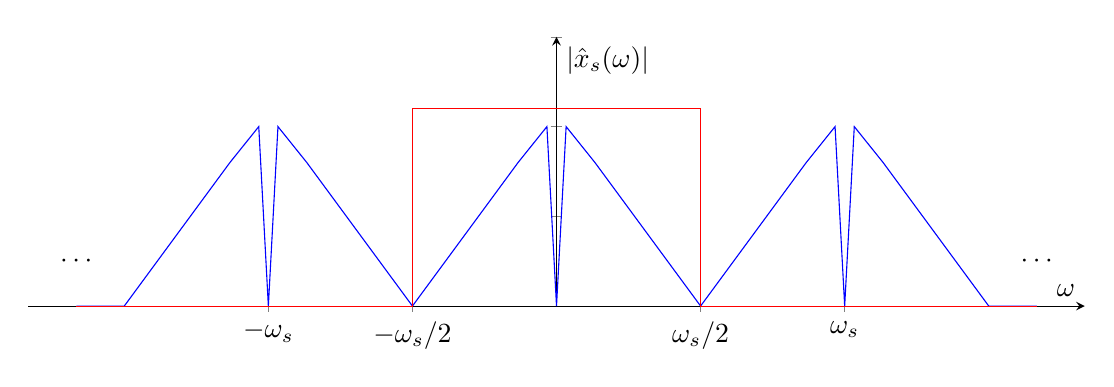
\begin{tikzpicture}
    \begin{axis}[width=15cm,height=5cm,ymin=0,ymax=3,
        xmin=-11,xmax=11,
        xlabel={$\omega$},
        ylabel={$|\hat{x}_s(\omega)|$},
        axis x line=center,
        axis y line=center,
        yticklabels={,,,},
        xtick={-6,-3,3,6},
        xticklabels={$-\omega_s$,$-\omega_s/2$,$\omega_s/2$,$\omega_s$}
      ]
      \addplot[mark=none,color=blue] plot coordinates {(-10,0.0) (-9.0,0) (-6.8,2*0.8) (-6.2,2*1) (-6,0) (-5.8,2*1) (-5.2,2*0.8) (-3,0) (-3,0) (-0.8,2*0.8) (-0.2,2*1) (0,0) (0.2,2*1) (0.8,2*0.8) (3,0)  (3,0) (5.2,2*0.8) (5.8,2*1) (6,0) (6.2,2*1) (6.8,2*0.8) (9,0) (10,0) } ;
      \draw node at (axis cs:-10,0.5) {$\cdots$};
      \draw node at (axis cs:10,0.5) {$\cdots$};
      \draw node at (axis cs:3.5,2.5) {$\Hiw$};
      \addplot[mark=none,color=red] plot coordinates {(-10,0.0) (-3,0) (-3,2.2) (3,2.2) (3,0) (10,0) } ;

      %    \addplot[mark=none,color=blue] plot coordinates {(-10,0.0) (-7,0) (-6.8,2*0.8) (-6.2,2*1) (-6,0) (-5.8,2*1) (-5.2,2*0.8) (-5,0) (-1,0) (-0.8,2*0.8) (-0.2,2*1) (0,0) (0.2,2*1) (0.8,2*0.8) (1,0)  (5,0) (5.2,2*0.8) (5.8,2*1) (6,0) (6.2,2*1) (6.8,2*0.8) (7,0) } ;
    \end{axis}
  \end{tikzpicture}
  \begin{tikzpicture}
    \begin{axis}[width=15cm,height=5cm,ymin=0,ymax=3,
        xmin=-11,xmax=11,
        xlabel={$\omega$},
        ylabel={$|\hat{x}(\omega)|$},
        axis x line=center,
        axis y line=center,
        yticklabels={,,,},
        xtick={-6,-3,3,6},
        xticklabels={$-\omega_s$,$-\omega_s/2$,$\omega_s/2$,$\omega_s$}
      ]
      \addplot[mark=none,color=blue] plot coordinates {(-10,0.0)  (-3,0) (-0.8,2*0.8) (-0.2,2*1) (0,0) (0.2,2*1) (0.8,2*0.8) (3,0)   (10,0) } ;

      ;
    \end{axis}
  \end{tikzpicture}
\end{center}
This is in essence the proof of Shannon's sampling theorem. To obtain $x(t)$, 
one can use an inverse Fourier transform:
\begin{equation}
  x(t) = \frac{1}{2\pi}\int_{-\infty}^{\infty} \hat{x}(\omega) e^{i\omega t}d\omega.
\end{equation}
If $\hat{x}_s(\omega)$ contains overlapping copies of $\hat{x}(\omega)$, then the original 
spectrum $\hat{x}(\omega)$, and therefore the original signal $x(t)$, cannot be reconstructed.

For a complex-valued signal, we would need to apply an ideal band-pass filter, which only 
retains signals between $\omega_{\mathrm{min}}$ and
$\omega_{\mathrm{max}}$, instead of the ideal low-pass filter. The same applies to an undersampled signal.

\subsection{Ideal reconstruction filter}
Recall, from the beginning of this course, that we introduced the ideal reconstruction filter without deriving it. 
Now we can derive it. It is the inverse Fourier transform of the ideal low-pass filter
\begin{equation}
  \Hiw = \left\{ \begin{array}{cc}
    T_s & |\omega| \le \frac{\omega_s}{2} \\
    0   & \mathrm{otherwise}
  \end{array}
  \right.
\end{equation}
which is
\begin{align}
  h(t) & = \frac{1}{2\pi}\int_{-\infty}^{\infty} \Hiw e^{i\omega t}d\omega                             \\
       & = \frac{1}{2\pi} \int_{-\omega_s/2}^{\omega_s/2} T_s e^{i\omega t}d\omega                     \\
       & = \frac{T_s}{2 \pi}\left. \frac{e^{i\omega t}}{it} \right|_{\omega=-\omega_s/2}^{\omega_s/2}  \\
       & = \frac{T_s}{2 t \pi i}\left( e^{i\frac{\omega_s}{2} t}  - e^{-i\frac{\omega_s}{2} t} \right) \\
       & = \frac{T_s}{\pi t} \sin(\frac{\omega_s}{2}t)                                                 
\end{align}
Keeping in mind that $\omega_s/2 = \pi/T_s$ we obtain the familiar result:
\begin{equation}
  \boxed{
    h(t) = \frac{T_s}{\pi t}\sin(\frac{\pi}{T_s}t)
  }
\end{equation}
When applying this reconstruction filter in time domain, one convolves the sampled signal to obtain the 
reconstructed continuous-time signal:
\begin{align}
  x(t) & = h(t)*x_s(t)                                                                                            \\
       & = \int_{-\infty}^{\infty} x_s(\tau)h(t-\tau)d\tau                                                        \\
       & = \int_{-\infty}^{\infty}\left( \sum_{n=-\infty}^{\infty} x[n] \delta(\tau-n T_s)\right) h(t-\tau) d\tau \\
       & = \sum_{n=-\infty}^{\infty} x[n] \int_{-\infty}^{\infty} \delta(\tau-nT_s) h(t-\tau)d\tau                \\
       & = \sum_{n=-\infty}^{\infty} x[n] \frac{\sin(\frac{\pi}{T_s}(t-n T_s))}{\frac{\pi}{T_s}(t-nT_s)}.
\end{align}
This reconstruction formula now perfectly reproduces $x(t)$ from
samples $x[n]$, provided that $\omega_s \ge 2\omega_{\mathrm{max}}$.

For an undersampled real-valued signal, or a complex-valued band limited signal, the ideal reconstruction 
filter would be different. In this case, it would correspond to the impulse response of an ideal band-pass filter.

